\documentclass[10pt]{beamer}
\usetheme{metropolis}
\usepackage{appendixnumberbeamer}
\usepackage{booktabs}
\usepackage[scale=2]{ccicons}
\usepackage{pgfplots}
\usepgfplotslibrary{dateplot}
\usepackage{xspace}
\newcommand{\themename}{\textbf{\textsc{metropolis}}\xspace}
%\includeonlyframes{}
%%%%%%%%%%%%%%%%%%%%%%%%%%%%%%%%%%%%%%%%%%%%%%%%%%%%%%%%%%%%%%%%%%%%%%%%%%%%%%%%
% Preambulo
%%%%%%%%%%%%%%%%%%%%%%%%%%%%%%%%%%%%%%%%%%%%%%%%%%%%%%%%%%%%%%%%%%%%%%%%%%%%%%%%
\usepackage[spanish,activeacute]{babel}
\usepackage{xcolor}
\usepackage{color}
\usepackage{colortbl}
\usepackage{amsmath}
\usepackage{amssymb}
\usepackage{graphicx}
\usepackage{latexsym}
\usepackage[T1]{fontenc}
\usepackage[utf8]{inputenc}
\usepackage{wrapfig}
\usepackage{siunitx}
\usepackage{times}
\usepackage{tikz}
\usepackage{verbatim}
\usepackage{multimedia}
\usepackage{hyperref}
\usepackage{thumbpdf}
\usepackage{pgf,pgfarrows,pgfnodes,pgfautomata,pgfheaps,pgfshade}
\usepackage{url}
\usepackage{empheq}
\usepackage{fancybox}
\usepackage{esint}
\usepackage{lipsum}
\usepackage{listings}
\usepackage{mathptmx}
\usepackage{helvet}
\usepackage{tikz}%
\usepackage{circuitikz}
\usepackage{csvsimple}
\usepackage{pgfplots}
\usepackage{multimedia}
\usepackage{media9}
\usepackage{proba}
\usepackage[absolute,overlay]{textpos}
\usepackage{bibunits}
\usepackage{tcolorbox}
%\usepackage[texcoord,grid,gridunit=mm,gridcolor=red!
%60,subgridcolor=green!60]%
%{eso-pic}
\pgfplotstableread[col sep = comma]{./IMAGENES/gbm.csv}\mydata
\usepackage[makeroom]{cancel}
\usepackage{epstopdf}
\epstopdfsetup{outdir=./}
\title{Modelado con Ecuaciones Diferenciales
    Estoc\'asticas via Perturbaci\'on de Par\'ametros}
\subtitle{y una Invitaci\'on a la soluci\'on num\'erica de EDEs}
\date{Marzo 2--6, 2020}
\author{Sa\'ul D\'iaz Infante Velasco}
\institute{CONACYT-Universidad de Sonora}
%\titlegraphic{%
%\hfill\includegraphics[height=1.5cm]{./figures/logo_snidm.png}
%}
\metroset{block=fill}
%%%%%%%%%%%%%%%%%%%%%%%%%%%%%%%%%%%%%%%%%%%%%%%%%%%%%%%%%%%%%%%%%%%%%%%%%%%%%%%%
\def\Q#1#2{\frac{\partial #1}{\partial #2}}
\usetikzlibrary{arrows,shapes}
%%%%%%%%%%%%%%%%%%%%%%%%%%%%%%%%%%%%%%%%%%%%%%%%%%%%%%%%%%%%%%%%%%%%%%%%%%%%%%%%
%------------------------------------Theorems 
\theoremstyle{plain} % default
\newtheorem{Teorema}{Teorema}
\newtheorem{Ejemplo}{Ejemplo}
\theoremstyle{definition}
\newtheorem{Definicion}{Definici\'on}
\newtheorem{Corolario}{Corolario}
\newtheorem{Proposicion}{Proposici\'on}
\newtheorem{Prueba}{Prueba}
\theoremstyle{definition}
\newtheorem{definicion}{Definici\'on}
\newtheorem{lema}{Lema}
%-----------------------------ExtrasDeTercerPresentacion
%--------------------------------Fancyboxes-------------------------------------
\definecolor{myblue}{rgb}{.8, .8, 1}
\definecolor{shadecolor}{cmyk}{0,0,0.41,0}
\newcommand*\mybluebox[1]{%
	\colorbox{myblue}{\hspace{1em}#1\hspace{1em}}
}
\newcommand*\myyellowbox[1]{%
	\colorbox{darkyellow}{\hspace{1em}#1\hspace{1em}}
}
%--------------------------------------------------------------------------
\definecolor{shadecolor}{cmyk}{0,0,0.41,0}
\definecolor{light-blue}{cmyk}{0.25,0,0,0}
\newsavebox{\mysaveboxM} % M for math
\newsavebox{\mysaveboxT} % T for text
\newcommand*\Garybox[2][Example]{%
	\sbox{\mysaveboxM}{#2}%
		\sbox{\mysaveboxT}{\fcolorbox{black}{light-blue}{#1}}%
			\sbox{\mysaveboxM}{%
	\parbox[b][\ht\mysaveboxM+.5\ht\mysaveboxT+.5\dp\mysaveboxT][b]{%
		\wd\mysaveboxM}{#2}%
	}%
	\sbox{\mysaveboxM}{%
		\fcolorbox{black}{shadecolor}{%
		\makebox[\linewidth-10em]{\usebox{\mysaveboxM}}%
		}%
	}%
	\usebox{\mysaveboxM}%
	\makebox[0pt][r]{%
		\makebox[\wd\mysaveboxM][c]{%
			\raisebox{\ht\mysaveboxM-0.5\ht\mysaveboxT
			+0.5\dp\mysaveboxT-0.5\fboxrule}{\usebox{\mysaveboxT}}%
		}%
	}%
}
\newcommand\Fontvi{\fontsize{7}{7.2}\selectfont}
%%%%%%%%%%%%%%%%%%%%%%%%%%%%%%%%%%%%%%%%%%%%
\definecolor{kugreen}{RGB}{50,93,61}
\definecolor{kugreenlys}{RGB}{132,158,139}
\definecolor{kugreenlyslys}{RGB}{173,190,177}
\definecolor{kugreenlyslyslys}{RGB}{214,223,216}
\definecolor{greenArea}{RGB}{124,252,124}
\definecolor{hellmagenta}{rgb}{1,0.75,0.9}
\definecolor{hellcyan}{rgb}{0.75,1,0.9}
\definecolor{hellgelb}{rgb}{1,1,0.8}
\definecolor{colKeys}{rgb}{0,0,1}
\definecolor{colIdentifier}{rgb}{0,0,0}
\definecolor{colComments}{rgb}{1,0,0}
\definecolor{colString}{rgb}{0,0.5,0}
\definecolor{darkyellow}{rgb}{1,0.9,0}
\setbeamercovered{transparent}
\lstset{%
    language=[AlLaTeX]TEX,%
    float=hbp,%
    basicstyle=\ttfamily\small, %\usepackage{cir}
    identifierstyle=\color{colIdentifier}, %
    keywordstyle=\color{colKeys}, %
    stringstyle=\color{colString}, %
    commentstyle=\color{colComments}, %
    columns=flexible, %
    tabsize=3, %
    frame=single, %
    extendedchars=true, %
    showspaces=false, %
    showstringspaces=false, %
    numbers=left, %
    numberstyle=\tiny, %
    breaklines=true, %
    backgroundcolor=\color{hellgelb}, %
    breakautoindent=true, %
    captionpos=b,%
    xleftmargin=18pt,%
    xrightmargin=\fboxsep%
}
\pgfplotsset{
    left segments/.code={\pgfmathsetmacro\leftsegments{#1}},
    left segments=3,
    left/.style args={#1:#2}{
        ybar interval,
        domain=#1:#2,
        samples=\leftsegments+1,
        x filter/.code=\pgfmathparse{\pgfmathresult}
       }
}
\DeclareMathOperator{\sign}{sgn}
\newcommand{\innerprod}[2]{\left\langle#1, #2\right\rangle}
\newcommand\bound{10} % bound number of points on each side of N
\newcommand\labelnum[3][]{
	\begin{scope}[font=\footnotesize,x=.3cm,#1]
	  \foreach \mypt in {0,#2,...,\bound}{
	    \draw(\mypt,0)circle[radius=2pt];
	    \draw(-\mypt,0)circle[radius=2pt];
	  }
	  \draw(-\bound-5,0)--(\bound+5,0) node[pos=0, left]{$t$};
	  \node(start)[at={(-\bound-4,0)},label=below:{$t_0=0$}]{$[$};
	  \node(end)[at={(\bound+4,0)},label=below:{$T=Nh$}]{$]$};
	  \node[%
		  at={($(start)!.319!(end)$)},
		  label=below:{
			   $\underbrace{}_{h}$
			}%
			]{\vphantom{$[$}};
	  \node[at={($(start)!.57!(end)$)},label=below:{$t_{n+1}$}]{\vphantom{$[$}};
	  \filldraw(0,0)circle[radius=2pt];
	  \node[at={(-\bound-2,0)},above]{$\cdots$};
	  \node[at={(\bound+2,0)},above]{$\cdots$};
	  \node[at={(0,0)},above=5pt]{#3};
	\end{scope}
}
\tcbuselibrary{skins,breakable}

\defaultbibliography{CharlaBib}
\defaultbibliographystyle{abbrv}
\begin{document}
    \maketitle
    \section*{Introducci\'on}
        \begin{frame}
  \frametitle{Por que EDEs?}
	\begin{empheq}[box={\Garybox[En ocaciones]}]{align*}
		EDO+ruido=Mejor \text{ } modelo
	\end{empheq}
	\begin{overlayarea}{\textwidth}{.8\textheight}
		\begin{columns}
    		\column{.55\textwidth}
			\only<2-3>{
			\begin{exampleblock}{Crecimiento de Poblaciones}
				$$
					\frac{dN}{dt}=a(t)N(t) \qquad N_0=N(0)=cte.
				$$
			\end{exampleblock}
			}
			\only<4-8>{
			\begin{exampleblock}{Circuitos Eléctricos}
			\begin{align*}
				&L\cdot Q''(t)+
				R\cdot Q'(t)+
				\frac{1}{C}\cdot Q(t)
				=F(t)\\
				&Q(0)=Q_0\\
				&Q'(0)=I_0
			\end{align*}
		\end{exampleblock}
		}
		\only<7-8>{
		\begin{empheq}[box=\shadowbox*]{equation*}
			Q(t)=Z(t)+"ruido"
		\end{empheq}
		}
		\column{.58\textwidth}
		\only<3>{
			\begin{empheq}[box=\shadowbox*]{equation*}
				a(t)=r(t)+"ruido"
			\end{empheq}
		}
		\only<5-8>{
			%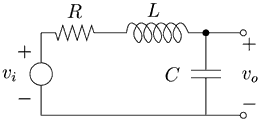
\includegraphics[width=\textwidth]{./images/CircuitRLC.png}
	     \begin{circuitikz}[american voltages]
	      \draw (0,0)
      		to[sV,v=$F(t)$] (0,2) % The voltage source
      		to[R=$R$, i^>=$i(t)$] (2,2) % The resistor
          to[L=$L$] (4,2)
          to[C=$C$] (4,0)
          --(0,0) ;
			\end{circuitikz}
		}
		\only<6-8>{
		\begin{empheq}[box=\shadowbox*]{equation*}
			F(t)=G(t)+"ruido"
		\end{empheq}
		}
		\only<8>{
			Estima $Z(t)$ observando $Q(t)$
		}
	\end{columns}
	\end{overlayarea}
\end{frame}
%%%%%%%%%%%%%%%%%%%%%%%%%%%%%%%%%%%%%%%%%%%%%%%%%%%%%%%%%%%%%%%%%%%%%%%%%%%%%%%%%
\begin{frame}
  \frametitle{Para fijar ideas}
  \begin{empheq}[box={\Garybox[Ejemplo]}]{align*}
 		dN(t) = aN(t)dt
 	\end{empheq}
   \begin{overlayarea}{\textwidth}{.3\textheight}
     \begin{columns}
       \column{.5\textwidth}
        \only<2->{
          \begin{block}{Perturba sobre $[t, t+dt)$}
            \only<3->{
            $$
              a dt
              \rightsquigarrow
              a dt + \sigma dB(t)
            $$
            }
           \end{block}
		       }
        \column{.5\textwidth}
          \only<4->{
            \begin{exampleblock}{obten una EDE}
              $$
               dN(t) = aN(t)dt + \sigma N(t) dB(t)
              $$
            \end{exampleblock}
            }
     \end{columns}
   \end{overlayarea}
  \begin{overlayarea}{\textwidth}{.7\textheight}
    \centering
    \resizebox{0.45\textwidth}{!}{%
     \only<5>{
     \begin{tikzpicture}
       \begin{axis}[%
         line width=1.0pt,
         mark size=1.0pt
         ]%
         \addplot [color=blue]%
         table [%
           x index = {0},
           y index = {1}
           ]{\mydata};
           \addplot[domain=0:5, samples=100]{1.5*exp(x)};
       \end{axis}
     \end{tikzpicture}
     }
  }
  \end{overlayarea}
\end{frame}
%%%%%%%%%%%%%%%%%%%%%%%%%%%%%%%%%%%%%%%%%%%%%%%
 \begin{frame}
 	\frametitle{¿Por que hacer métodos numéricos para EDEs?}
 	\begin{empheq}[box={\Garybox[En ocaciones]}]{align*}
 		EDO+ruido=Mejor \text{ } modelo
 	\end{empheq}
 	\begin{overlayarea}{\textwidth}{.7\textheight}
 		\begin{columns}
     		\column{.5\textwidth}
 				\begin{alertblock}{Solución analítica?}
 					muy RARA
 				\end{alertblock}
 			\column{.5\textwidth}
 			\only<2>{
 				\begin{block}{Usa }
 					Teoría de diferencias finitas y haz una extención estocástica.
 				\end{block}
 			}
 		\end{columns}
 	\end{overlayarea}
 \end{frame}
 %%%%%%%%%%%%%%%%%%%%%%%%%%%%%%%%%%%%%%%%%%%%%%%%
 \begin{frame}
 	\frametitle{Objetivo}
 	\begin{alertblock}{Objetivo de la charla}
 		\textbf{Ilustrar} como aproximar soluciones de EDEs  a partir de
 \emph{conocimientos básicos}
 		de los \textbf{métodos deterministas} y nociones muy elementales de
variables 		 aleatorias.
 	\end{alertblock}
 \end{frame}
%%%%%%%%%%%%%%%%%%%%%%%%%%%%%%%%%%%%%%%%%%%%%%%%%%%%%%%%%%%%%%%%%%%%%%%%%%%%%%

%   %\section{}
%%%%%%%%%%%%%%%%%%%%%%%%%%%%%%%%%%%%%%%%%%%%%%%%%%%%%%%%%%%%%%%%%%%%%%%%%%%%%%%%%
    \begin{frame}{Esquema de Charla}
        \setbeamertemplate{section in toc}[sections numbered]
        \tableofcontents[hideallsubsections]
    \end{frame}
    \section{Construcción de Métodos Numéricos}
        \subsection{EDEs en sentido de It^o}
            \begin{frame}
  \frametitle{Notación}
  \begin{empheq}[box={\Garybox[
		\hyperlink{thm:ExistenciaUnicidadEDE}{EDE}]}
  ]{align*}
    \only<1-3>{
    dx(t)&= 
 			\underbrace{f(x(t),t)dt}_{\text{deriva}} 
 			+
 			\underbrace{g(x(t),t) dB(t)}_{\text{difusión}},\\
	  }
	  \only<2-3>{
				x_0 &= x(0), \quad
				t\in[0,T].\\
			}
 	  \only<4>{
 	  x(t) &= x_0 + \int_0^t f(x(s),s)ds
		  +
		  \int_0^t g(x(s),s)dB(s)
 	  }
  \end{empheq}
	\hypertarget<4>{frm:notacion}
	\only<3->{
		\begin{align*}
			&f:\R ^d 
				\times [0,T] \to \R^d,
			\qquad
			g:\R^d 
				\times [0,T] \to \R^{d\times m} \\
			&B(t)=\left(B_1(t),\dots,B_m(t)\right)^T,
			\quad
			\left(
				\Omega, \calF, \{\calF_t\}_{t\geq 0}, \P
			\right)
		\end{align*}
	}
\end{frame}

            \begin{frame}
   \frametitle{Idea general de la construcción}
  \begin{empheq}[box={\Garybox[EDE]}]{align*}
 	  x(t) &= x_0 + \int_0^t f(x(s),s)ds
		  +
		  \int_0^t g(x(s),s)dB(s)
	\end{empheq}
	\only<2->{
	\centering
		\begin{tikzpicture}
		  \labelnum[yshift=-2cm]{2}{Stencil}
		\end{tikzpicture}
	}
 	\only<3>{
		\begin{equation*}
			x(t_{n+1}) = 
			x(t_{n}) 
			+
			\int_{t_{n}}^{t_{n+1}} f(x(s),s)ds
		  +
		  \int_{t_{n}}^{t_{n+1}} g(x(s),s)dB(s)
		\end{equation*}
	}
	\only<4-6>{
		\begin{equation*}
			x(t_{n+1}) = 
			x(t_{n}) 
			+
			\underbrace{
				\int_{t_{n}}^{t_{n+1}} f(x(s),s)ds
		  }_{%
				  \textcolor<5-6>{red}{%
					  \approx \text{det}%
					 }
				}
		  +
		  \underbrace{
			  \int_{t_{n}}^{t_{n+1}} g(x(s),s) dB(s)
			}_{%
					\textcolor<6>{red}{%
						\hyperlink{frm:integracion}{\approx}
						}
				}
		\end{equation*}
	}
	\hypertarget<6>{frm:incremento_bm}{}
	\only<7->{
		\begin{equation*}
			x(t_{n+1}) = 
			x(t_{n}) 
			+
			\underbrace{
				\int_{t_{n}}^{t_{n+1}} f(x(s),s)ds
		  }_{%
				  \textcolor{red}{%
					  \approx 
					   f(x_n) h
					 }
				}
		  +
		  \underbrace{
			  \int_{t_{n}}^{t_{n+1}} g(x(s),s)dB(s)
			}_{
				\substack{
					\approx 
					g(x_n) \Delta B_n \\
					\Delta B_n = B_{t_{n+1}}-B_{t_n}
				}
			}
		\end{equation*}
	}
	\only<7>{
		\begin{textblock*}{.25\textwidth}(4.5cm,3.0cm)
			\begin{exampleblock}{}
				% left hand sums
				\centering
				\begin{tikzpicture}[scale=0.3,%
				/pgf/declare function={f=-15*(x-5)+(x-5)^3+50;}]
					\begin{axis}[
					        xmin=0,xmax=8,ymin=0,ymax=80,
					    domain=0:10,
					    samples=100,
					    axis lines=middle
					]
					\addplot [thick, red] {f};
					\addplot [
					    black!80,fill=green,opacity=.3,
					    left segments=7,
					    left=1:6
					] {f};
					\end{axis}
				\end{tikzpicture}
			\end{exampleblock}
		\end{textblock*}
	}
 	\only<8>{
		\begin{align*}
				X_0 &=x_0, \qquad X_n  \approx x(t_n),
				\qquad 
				n=1 \dots, N-1
				\\
				X_{n+1} &= X_n + f(X_n) h + g(X_n) \Delta B_n, 
		 \end{align*}
	}
 	\only<9>{
 		\begin{align*}
 			X_0 &=x_0, \qquad X_n  \approx x(t_n),
 			\qquad 
 			n=1 \dots, N-1
 			\\
 			X_{n+1} &= X_n + f(X_n) h + g(X_n) 
 			\textcolor{blue}{%
 				\underbrace{\Delta B_n}_{%
 					\approx
 				}%
 			}%
 	 \end{align*}
 	}
\end{frame}

        \subsection{Aproximaci\'on de Movimiento Browninano}
            %%%%%%%%%%%%%%%%%%%%%%%%%%%%%%%%%%%%%%%%%%%
	\begin{frame}{Historia}
		\begin{center}
			\movie[width=9.1cm,%
				height=5.2cm,%
				showcontrols=true,%
				loop,poster]{}{BrownianMotion.flv}
			\end{center}
		\end{frame}
%%%%%%%%%%%%%%%%%%%%%%%%%%%%%%%%%%%%%%%%%%%
\begin{frame}{Caminata del borracho}
	\centering
	\begin{tikzpicture}[
    ,
    axis/.style={thick, ->, >=stealth'},
    pile/.style={%
    	line width=1.0mm,
        ->, 
        >=stealth', 
        color = black!45!green
    	},
    every node/.style={%
    	color=black!40!blue
	   }
    ]
    % axis
    \draw[step=1cm,gray,very thin] (-1,-1) grid (6,6);
    \draw[axis] (-1,0)  -- (6,0) node(xline)[right]
        {$t$};
    \draw[axis] (0,-1) -- (0,6) node(yline)[above] {$X$};
    % Lines
    \draw[pile] (0,0) coordinate (A) -- (0,1)
        coordinate (B) node[right, text width=10em] {$\P[X_n=\pm 1]=1/2$};
    \draw[pile] (0,0) coordinate (C) -- (1,0)
        coordinate (D) node[below, text width=4em] {1}; 
	\end{tikzpicture}
\end{frame}
%%%%%%%%%%%%%%%%%%%%%%%%%%%%%%%%%%%%%%%%%%
\begin{frame}{Caminata Aleatoria}
	\begin{overlayarea}{\textwidth}{.7\textheight}
	\only<1>{
	\begin{center}
		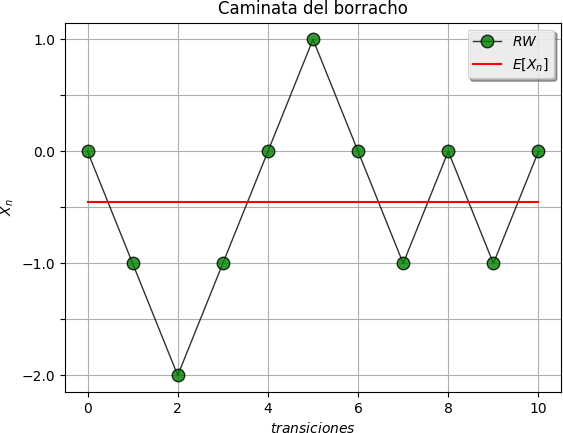
\includegraphics[width=.9\textwidth]{./IMAGENES/RW/RandomWalk_1_.png}
	\end{center}
	}
	\only<2>{
		\begin{center}
			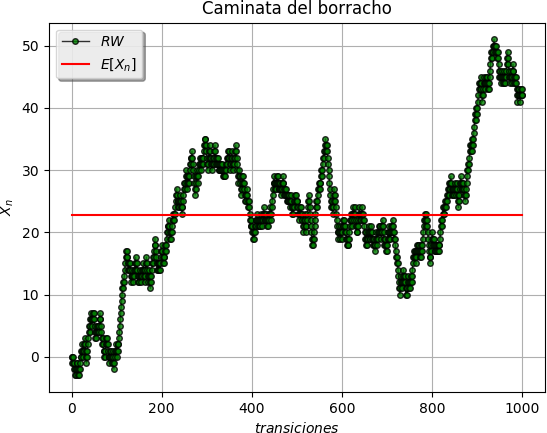
\includegraphics[width=0.83\textwidth]{./IMAGENES/RW/RandomWalk_2_.png}
		\end{center}
	}
	\only<3>{
		\begin{center}
			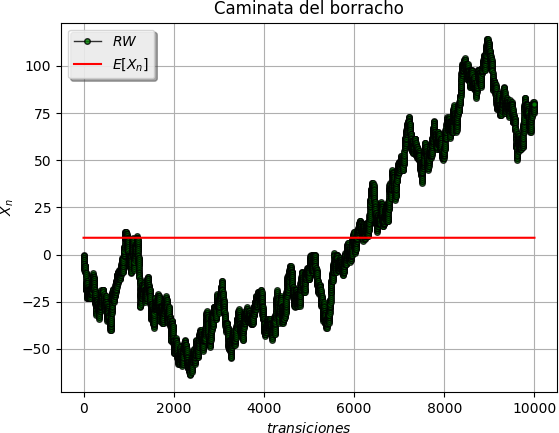
\includegraphics[width=0.83\textwidth]{./IMAGENES/RW/RandomWalk_3_.png}
		\end{center}
	}
	\end{overlayarea}
\end{frame}
%%%%%%%%%%%%%%%%%%%%%%%%%%%%%%%%%%%%%%%%%%%%%%%%%%%%%%%%%%%%%%%%%%%%%%%%%%%%%%%%
%%%%%%%%%%%%%%%%%%%%%%%%%%%%%%%%%%%%%%%%%%%%%%%%%%%%%%%%%%%%%%%%%%%%%%%%%%%%%%%%
\begin{frame}{Caminata del borracho}
	\centering
	\begin{tikzpicture}[
    scale=1,
    axis/.style={thick, ->, >=stealth'},
    pile/.style={%
    	line width=1.0mm,
        ->, 
        >=stealth', 
        color=black!45!green
    	},
    every node/.style={%
    	color=black!40!blue
	   }
    ]
    \draw[step=1cm,gray,very thin] (-1,-1) grid (6,6);
    \draw[axis] (-1,0)  -- (6,0) node(xline)[right]
        {$t$};
    \draw[axis] (0,-1) -- (0,6) node(yline)[above] {$Y_n$};
    \draw[pile] (0,0) coordinate (A) -- (0,1)
        coordinate (B) node[right, text width=10em] {%
        $\P[X_n=\pm \varepsilon]=1/2$%
        };%
    \draw[pile] (0,0) coordinate (C) -- (1,0)
        coordinate (D) node[below, text width=4em] {$\delta$}; 
	\end{tikzpicture}
\end{frame}
%%%%%%%%%%%%%%%%%%%%%%%%%%%%%%%%%%%%%%%%%%%%%%%%%%%%%%%%%%%%%%%%%%%%%%%%%%%%%%%
\begin{frame}{Construcci\'on}
	\begin{columns}
		\column[t]{.5\textwidth}
		\begin{overlayarea}{\textwidth}{\textheight}
			\only<2->{
				\begin{empheq}{align*}
					&\{ X_{n} \}_{n=1}^{\infty}   \quad v.a. .i.d\\
					&P(X_{j} = \pm \varepsilon)= \frac{1}{2}.
				\end{empheq}
			}
			\only<3->{
				\begin{empheq}[box=\shadowbox*]{align*}
					Y_{\delta, \varepsilon}(0) = &0\\
					Y_{ \delta, \varepsilon}(n \delta )= 
					&
					X_{1} + X_{2} + \cdots + X_{n}.
				\end{empheq}
			}
			\only<4->{
				Interpola linealmente
				\begin{empheq}{align*}
					Y_{\delta, \varepsilon}(t) =
						&
							\frac{(n + 1) \delta - t}{\delta} 
							Y_{\delta, \varepsilon} (n \delta)
						\\
					 +
					 &
						 \frac{t - n \delta}{\delta}
						 Y_{\delta, \varepsilon}
						\left(
							 (n+1) \delta
						\right).
					\\
					&
						n \delta < t < (n + 1) \delta .
				\end{empheq}
				}			
		\end{overlayarea}
	\column[t]{.6\textwidth}
		\begin{overlayarea}{\textwidth}{\textheight}
			\only<5->{
				\begin{alertblock}{Queremos}
					 $$
						\lim_{
							\substack{
								\delta\to 0\\
								\varepsilon \to 0
							}
						}
					 	Y_{\delta, \varepsilon}
					 $$
				\end{alertblock}
			}
			\only<6>{
				Tomate
		 		$
					\lambda \in \mathbb{R}
				$ fijo. Calcula
		 		\\
		 		\hyperlink{dfn:FuncionCaracteristica}{\beamergotobutton{caracteristica}}
				$
					\displaystyle
					\lim_{\delta, \varepsilon \to 0}
					\mathbb{E}
					\left[
						e^{ 
							i \lambda 
							Y_{\delta, \varepsilon}(t)
						}
					\right]
				$.
				\\
				\hypertarget{cns:Limite}{}
			}
			\only<7->{
				\textcolor<7>{red}{$t=n\delta$},
			}
			\only<7>{
				\begin{align*}
					\EX{
						e^{
							i\lambda
							Y_{\delta, \varepsilon}(\textcolor{red}{t})
						}
					}
					&=
					\prod_{j=1}^{n}
					\EX{
						e^{%
							i \lambda X_{j}%
						}
					}
					\\
					&=
					\left( 
						\EX{
							e^{i\lambda X_{j}}
						}
					\right)^{n}
					\\
					&=
					\left(
						\frac{1}{2} 
							e^{i \lambda \varepsilon}
					+
						\frac{1}{2}
							e^{-i \lambda \varepsilon}
					\right)^{n}
					\\
					&=
					\left(
						\cos(\lambda h)
					\right)^{n}\\
					&=
					\left(
						\textcolor{blue}{\cos(\lambda h)}
					\right)^{
									\frac{t}{
										\textcolor{blue}{\delta}
									}
							}.
				\end{align*}
			}
			\only<8->{
				\textcolor{cyan}{
					$
						u =
						\left(
							cos(\lambda \varepsilon)
						\right)^{\frac{1}{\delta}}
					$
				}
			}
			\only<9-10>{
				$
					\ln(u)= \frac{1}{\delta} 
					\ln(cos(\lambda \varepsilon))
				$
				\\
				Para $x$ chirris!!!
				$
					\ln(1+x)\approx x 
				$
				\\
				Para $\varepsilon$ chirris!!!
				$
					\cos(\lambda \epsilon)
					\approx 
					1 - \frac{1}{2} \lambda^2 \varepsilon^2	
				$.
				Entonces
			}
			\only<11-12>{
				\begin{empheq}{align*}
					u \approx 
						& 
						e^{ 
							- \frac{1}{2\delta}
							\lambda^{2}
							\varepsilon^{2}
						}
					\\
					\EX{
						e^{ 
							i \lambda 
							Y_{\delta, \varepsilon}(t)
						}
					}
					\approx &
					e^{
						- \frac{1}{
								2
								\textcolor{red}{\delta}
						}
						 t\lambda^{2}
						\textcolor{red}{\varepsilon}^{2}
					}.
			\end{empheq}
			}
			\only<11->{
				\textcolor{red}{$\varepsilon^{2} = \delta$}
			}
			\only<11->{
				$$
					\displaystyle
					\lim_{
						\delta \to 0 
					}
					\EX{
						e^{
							i \lambda 
							Y_{\delta, \sqrt{\delta}} (t)
						}
					}
					= 
					e^{ 
						-\frac{1}{2} t 
						\lambda^{2}
					},
					\qquad \lambda \in \mathbb{R}.
				$$
			}				\only<12>{
		 			\begin{empheq}[box=\ovalbox]{equation*}
		 			\therefore
		 			B(t)
		     			\overset{ \mathcal{D} }{ = }
		   				\displaystyle
		   				\lim_{\delta \to 0}
								Y_{\delta, \sqrt{\delta}}(t)
		 			\end{empheq}
				}
			\end{overlayarea}
		\end{columns}
	
\end{frame}
%%%%%%%%%%%%%%%%%%%%%%%%%%%%%%%%%%%%%%%%%%%%%%%%%%%%%%%%%%%%%%%%%%%%%%%%%%%%%%%
\begin{frame}{Construcci\'on}
	\begin{Teorema}
		Sea $Y_{\delta, \varepsilon}(t)$ una caminata aleatoria que inicia en $0$
		de saltos $\varepsilon$ y $-\varepsilon$  
		con igual probabilidad en los tiempos
		$\delta, 2\delta,3\delta, \ldots $.
		Supongamos que $\varepsilon^{2} = \delta$.
		Entonces para cada $t \geq 0$, el limite
		$$ 
			B(t) = \displaystyle
			\lim_{\delta \to 0}
			Y_{\delta, \sqrt{\delta}}(t),
		$$
		existe en distribución. Además, 
		$$
			\mathbb{E}\left[e^{i\lambda B(t)}\right]
				= e^{- \frac{1}{2}t\lambda^{2}}, \quad \quad \lambda \in 	\mathbb{R}.
		$$
	\end{Teorema}
\end{frame}
%%%%%%%%%%%%%%%%%%%%%%%%%%%%%%%%%%%%%%%%%%%%%%%%%%
\begin{frame}{Código}
	\only<+>{
  	\begin{figure}
  	\centering
      \tiny
   	\lstset{language=python}
         \lstinputlisting[firstline=3,lastline=11]{RW01.py}
   \end{figure}
}
\end{frame}
%%%%%%%%%%%%%%%%%%%%%%%%%%%%%%%%%%%%%%%%%%%
\begin{frame}{Caminata Aleatoria de $n$  transiciones}
	\begin{overlayarea}{\textwidth}{.7\textheight}
	\only<1>{
		\begin{center}
			\includegraphics[width=.85\textwidth,keepaspectratio]%
			{./IMAGENES/RW/RW01_1_.png}
		\end{center}
	}
	\only<2>{
		\begin{center}
			\includegraphics[width=.85\textwidth,keepaspectratio]%
			{./IMAGENES/RW/RW01_2_.png}
		\end{center}
	}
	\only<3>{
		\begin{center}
			\includegraphics[width=.85\textwidth,keepaspectratio]%
			{./IMAGENES/RW/RW01_3_.png}
		\end{center}
	}
	\end{overlayarea}
\end{frame}
%%%%%%%%%%%%%%%%%%%%%%%%%%%%%%%%%%%%%%%%%%%%%%%%%%%%%%%%%%%%%%%%%%%%%%%%%
\begin{frame}{Construcci\'on}
	\begin{empheq}[box={\Garybox[Construcci\'on]}]{align*}
		\varepsilon^{2} 
		& =
			\delta
		\\
		Y_{\delta, \varepsilon}(t)
		& 
			\xrightarrow[\delta, \varepsilon \to 0]{%
				\mathcal{D}
			} B(t) 
			\qquad \forall t 
			\geq 0
			\\
		\EX{
			e^{i\lambda B(t)}
		}
		&
		\xrightarrow{\delta ,\varepsilon \to 0}
			e^{
				-\frac{1}{2}t
				\lambda^{2}
			}, \quad \lambda \in 	\mathbb{R}.
	\end{empheq}
\end{frame}
%%%%%%%%%%%%%%%%%%%%%%%%%%%%%%%%%%%%%%%%%%%%%%%%%%
\begin{frame}{Distribuci\'on Gaussiana}
	\begin{figure}
		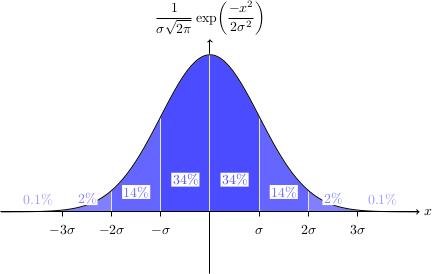
\includegraphics[width=\textwidth]{%
			./IMAGENES/RW/Standard_deviation_diagram.png%
		}
	\end{figure}
\end{frame}
%%%%%%%%%%%%%%%%%%%%%%%%%%%%%%%%%%%%%%%%%%%%%%%%%%%%%%%%%%%%%%%%%%%%%%%%%%
\begin{frame}{Caminata Aleatoria en $[0,1]$}
	%\vspace{-1.5cm}
	\begin{overlayarea}{\textwidth}{.7\textheight}
	\only<1>{
		\begin{center}
			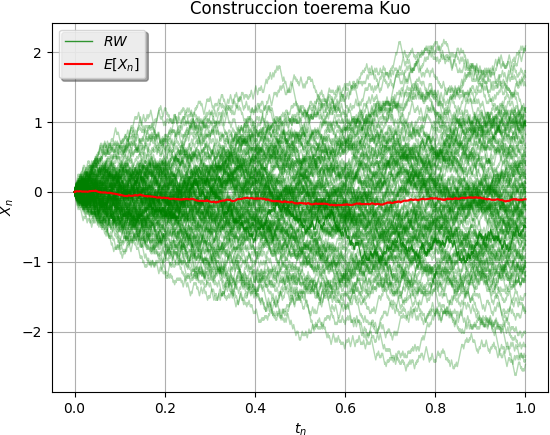
\includegraphics[width=.8\textwidth]{./IMAGENES/RW/RWs01.png}
		\end{center}
	}
	\only<2>{
		\begin{center}
			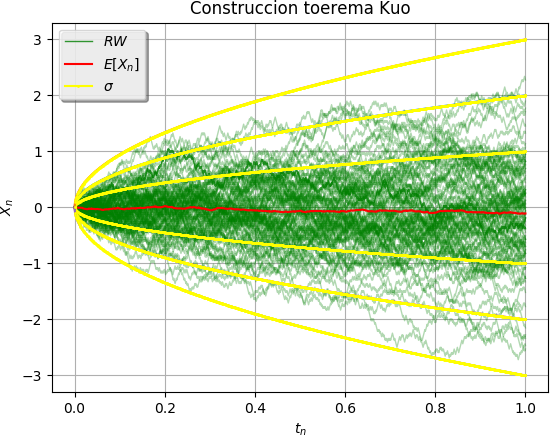
\includegraphics[width=.8\textwidth]{./IMAGENES/RW/RWs01Sigma.png}
		\end{center}
	}
	\end{overlayarea}
\end{frame}
%%%%%%%%%%%%%%%%%%%%%%%%%%%%%%%%%%%%%%%%%%%%%%%%%%%%%%%%%%%%%%%%%%%%%%%%%%%%%%%
\begin{frame}{Aproximación del MB en sentido Fuerte}
	\begin{definicion}
		El movimiento Browniano B(t) es el único proceso que satisface:
		\begin{enumerate}[(i)]
			\item 
				$B(0)=0$ c.s.
			\item 
				\textcolor<6>{orange}{
					Para $0\leq s \leq t$,
					$
						B(t) - B(s) \sim \sqrt{t-s} N(0,1).
					$
				}
			\item
				Para culquier $t_0 \leq t_1 \leq \dots \leq t_n \in [0,T]$, 
				las v.a
				$B(t_i)- B(t_j)$  son independientes 
		\end{enumerate}
	\end{definicion}
	\begin{overlayarea}{\textwidth}{0.5\textheight}
		\only<2-4>{
			Entonces, dados $t\in[0,T]$, y un stencil
			$$
				0=t_0\leq t_1 \leq \cdots \leq t_{M-1} \leq t_{M}=t
			$$
			\only<3>{
				$$
					B(t) = \sum_{j=1}^M 
						B(t_j)-B(t_{j-1}).
				$$
			}
			\only<4>{
			$$
				B(t) = \sum_{j=1}^M 
					\underbrace{
						B(t_j)-B(t_{j-1}).
					}_{:=\Delta B_j}
			$$
			}
		}
		\only<5-6>{
			Tomando $\{t_n\}_{n=0}^N$, $t_n = nh$, entonces
			$$
				B(t_n) \approx 
					\sum_ {j=0}^n \Delta B_j, 
					\qquad
					\Delta B_0:=0,
					\qquad
					\only<6>{
						\textcolor{orange}{
							\Delta B_j \sim \sqrt{h} N(0,1).
						}
					}
			$$	
		}
	\end{overlayarea}
\end{frame}
%%%%%%%%%%%%%%%%%%%%%%%%%%%%%%%%%%%%%%%%%%%%%%%%%%%%%%%%%%%%%%%%%%%%%%%%%%%%%%%%

        \subsection{Construcci\'on del Euler-Mayurama}
        \section{Aproximaci\'on Fuerte vs. D\'ebil}
            \begin{frame}
  \frametitle{Debil vs Fuerte}
  \begin{empheq}[box={\Garybox[dada]}]{align*}
 		dx(t)
			&=f(x(t))dt + g(x(t)) dB(t), 
 		\\
			x(0) &= x_0, \quad t\in[0,T]
 	\end{empheq}
  \begin{overlayarea}{\textwidth}{.7\textheight}
    \begin{columns}
      \column{.58\textwidth}
        \begin{block}{Debil}
          $$
						X_{n+1} = X_n + f(X_n) h 
							+ g(X_n) 
							\underbrace{\Delta B_n}_{%
								\substack{
									\approx \sqrt{h} \varepsilon_n\\
									\probX{\varepsilon_n=\pm 1}=1/2
								}
							}
					$$
        \end{block}
        %%%%%%%%%%%%%%%%%%%%%%%%%%%%%%%%
        \column{.58\textwidth}
          \begin{exampleblock}{Fuerte}
          $$
						X_{n+1} = X_n + f(X_n) h 
							+ g(X_n) 
							\underbrace{\Delta B_n}_{%
								\substack{
									\approx \sqrt{h} \epsilon_n\\
									\epsilon_n \sim N(0,1)
								}
							}
					$$
          \end{exampleblock}
    \end{columns}
  \end{overlayarea}
\end{frame}
    \section{Ejemplo: Reconstrucción de masa osea}
        %
%
% Esta parte funciona con Okular bajo linux.
% Para Windows, comentar el siguiente bloque y
% habilitar lo que sigue y presentar con acrobad reader
%
%
%
% %%%%%%%%%%%%%%%%%%%%%%%%%%%%%%%%%%%%%%%%%%%%%%%%%%
\begin{frame}{Proceso de Remodelación en BMU}
	\begin{tikzpicture}[remember picture,overlay]
	  \node[anchor=south west, inner sep=0pt] at (current page.south west) {%
    \movie[%
	    height = \paperheight,%
	    width = \paperwidth,%
	    poster,%
			showcontrols]{}{./Video/oc-ob.mp4}%
      };
  \end{tikzpicture}
\end{frame}
%%%Para windows (guacala!!!) es un purrun con el acrobad reader%%%
%\begin{frame}{Proceso de Remodelación en BMU}
%	\includemedia[
%	width=1\linewidth,height=0.6\linewidth,
%	activate=pageopen,
%	addresource=oc-ob.flv,        %adjust
%	flashvars={source=oc-ob.flv}  %adjust
%	]{\frame{Click!}}{VPlayer9.swf}
%\end{frame}
        %%%%%%%%%%%%%%%%%%%%%%%%%%%%%%%%%%%%%%%%%%%%%%%%%%%%%%%%%%%%%%%%5
\begin{frame}
	\frametitle{Fases de remodelación}
		\only<1-2>{%
			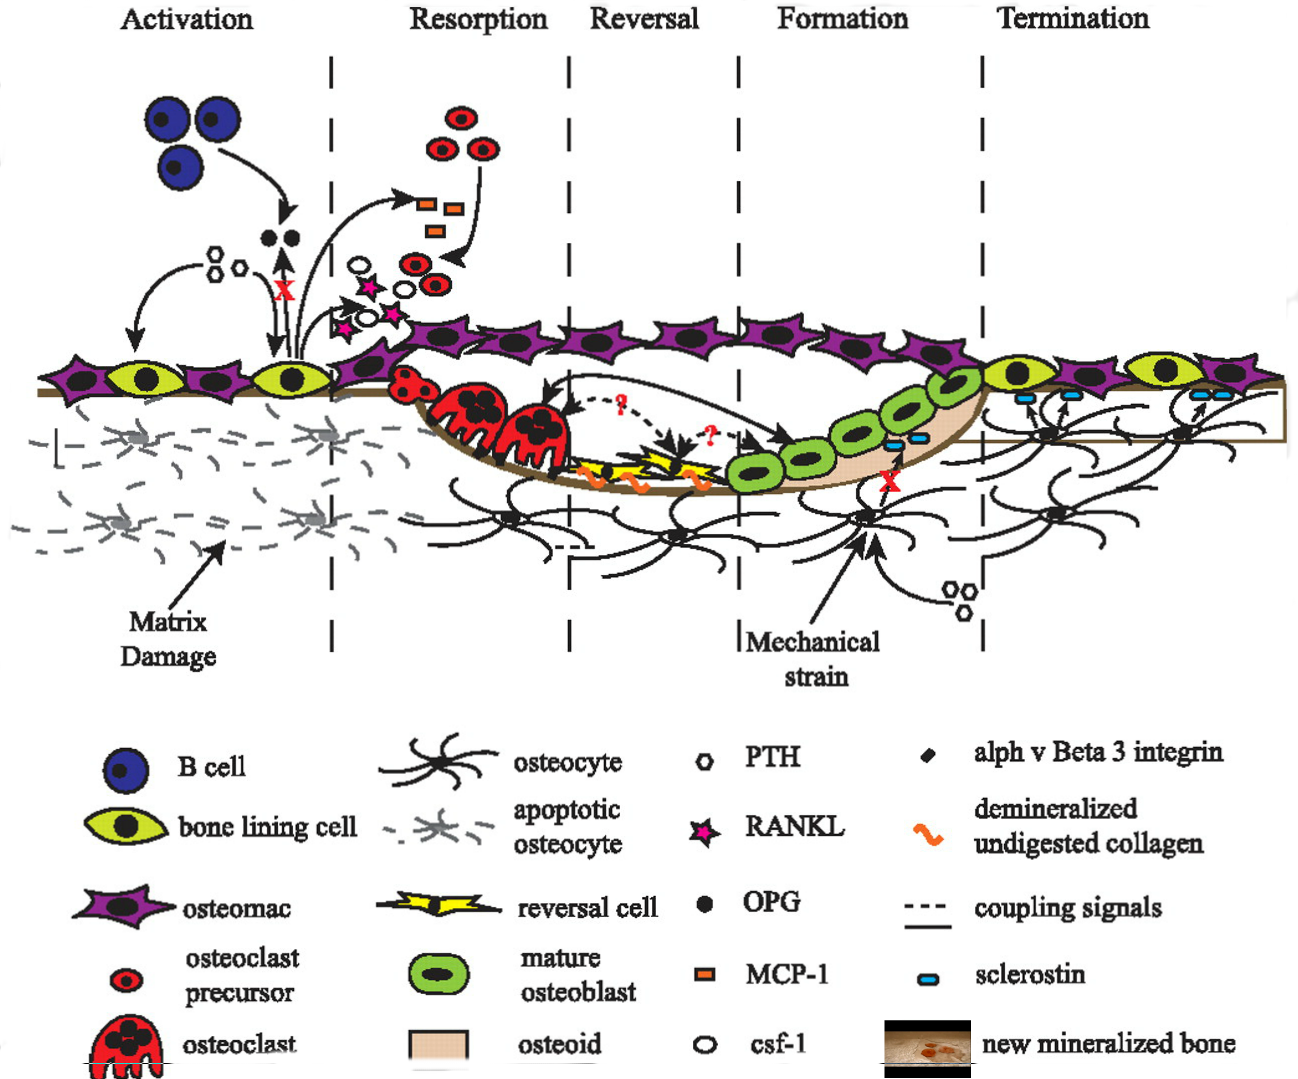
\includegraphics[width=\textwidth,keepaspectratio]{%
			./IMAGES/Komarova/boneRemodeling.png%
			}
		}
		\only<3-4>{%
			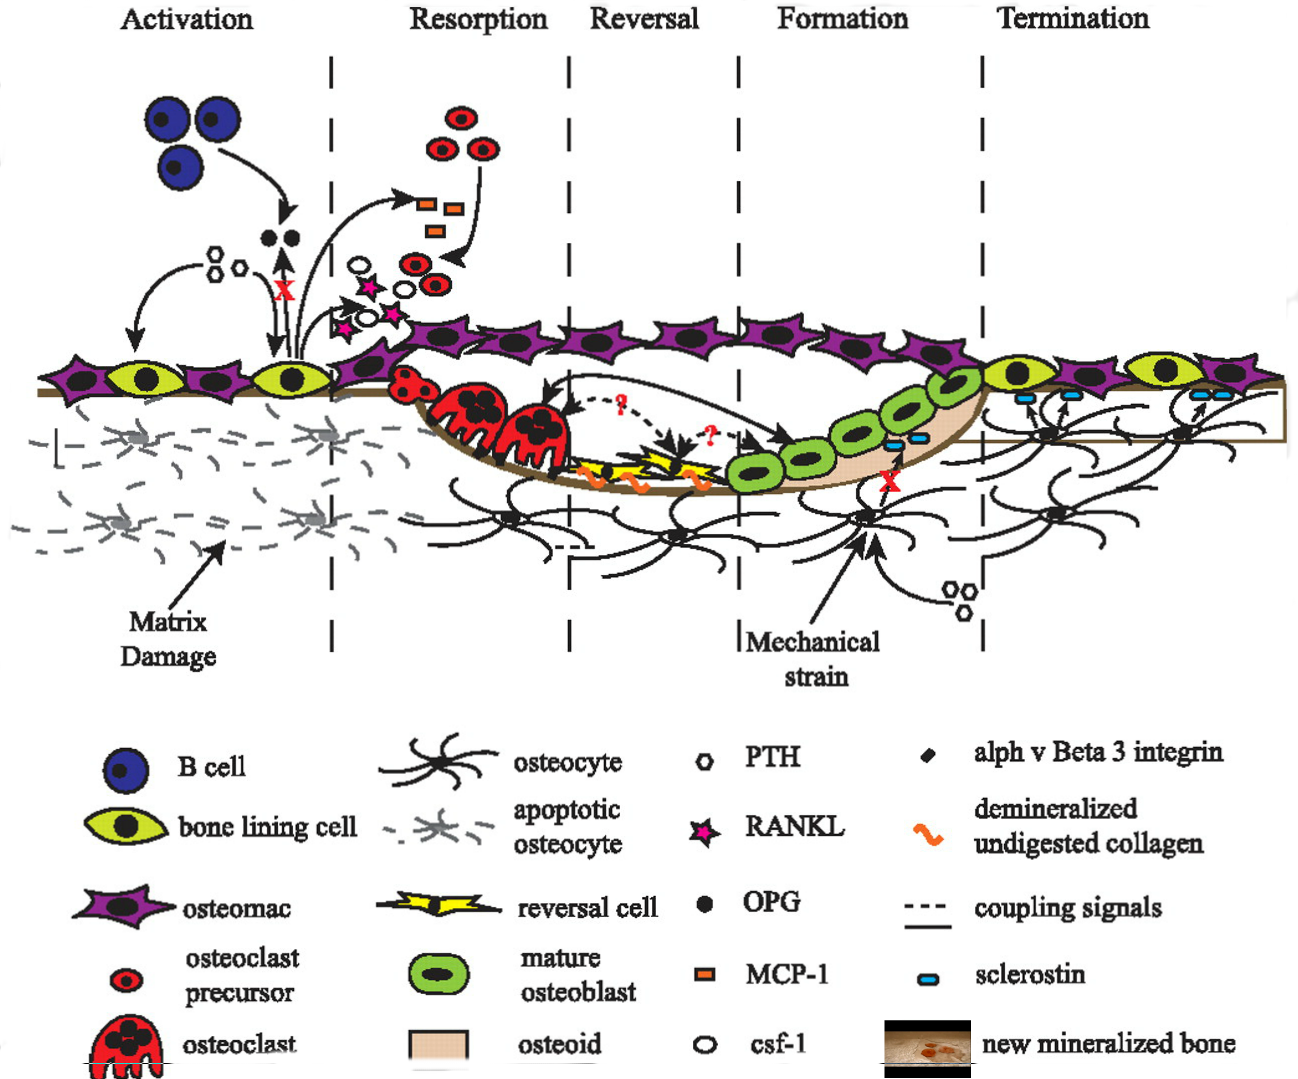
\includegraphics[width=.9\textwidth,keepaspectratio]{%
			./IMAGES/Komarova/boneRemodeling.png%
			}
		}

 		\only<1-2>{
			\begin{textblock*}{105mm}(10mm, 70mm)
				\begin{block}{Fases del proceso de remodelación}
						\begin{bibunit}[apalike]
						\nocite{Raggatt2010}
						\putbib
					\end{bibunit}
				\end{block}
			\end{textblock*}
 		}
\end{frame}

        \begin{frame}{}
	\frametitle{El Modelo de Komarova}
 	\only<1->{
		\begin{textblock*}{40mm}(10mm, 20mm)
			\begin{align*}
 			\frac{du}{dt} &=
 				u^{\kappa_1}
				\left(
					\alpha_1 v^{\gamma_1} - \beta_1
				\right)
				\\
			\frac{dv}{dt} &=
				v^{\kappa_2}
				\left(
					\alpha_2 u^{\gamma_2} - \beta_2
				\right)
			\\
			\only<3->{
					\frac{dz}{dt} &=
				-
				k_1 \max\{u - \widetilde{u}, 0\}
				\\
				&
				+
				k_1 \max\{v - \widetilde{v}, 0\}
			}
				\end{align*}
		\end{textblock*}
 	}
	\only<4>{% modelote
		\begin{textblock*}{.9\textwidth}(10mm, 5mm)
			\begin{exampleblock}{Descripción}
				\includegraphics[width=.98\textwidth, keepaspectratio]%
				{./IMAGES/Komarova/komarovaModelDescripcion.png}
			\end{exampleblock}
		\end{textblock*}	
	}
	\only<5>{% modelote
		\begin{textblock*}{.9\textwidth}(10mm, 5mm)
			\begin{exampleblock}{Descripción}
				\includegraphics[width=.98\textwidth, keepaspectratio]%
				{./IMAGES/Komarova/komarovaModelDescripcionb.png}
			\end{exampleblock}
		\end{textblock*}	
	}
	%
	\only<6>
	{
		\begin{textblock*}{.5\textwidth}(60mm, 20mm)
			\includegraphics[width=\textwidth, keepaspectratio]%
			{./IMAGES/Komarova/komarovaModel1.png}
		\end{textblock*}
	}
	\only<2-4>{
		\begin{textblock*}{100mm}(10mm, 63mm)
			\begin{bibunit}[alpha]
				\nocite{Komarova2003}
				%\biblio{CharlaBib.bib}
				\putbib
		  \end{bibunit}
  \end{textblock*}
	}
\end{frame}

        \begin{frame}{}
	\frametitle{Simplificación}
 	\only<1->{
		\begin{textblock*}{40mm}(10mm, 20mm)
			\begin{align*}
				\only<1>{
					\frac{du}{dt} &=
						u^{\kappa_1}
						\left(
							\alpha_1 v^{\gamma_1} - \beta_1
						\right)
						\\
					\frac{dv}{dt} &=
						v^{\kappa_2}
						\left(
							\alpha_2 u^{\gamma_2} - \beta_2
						\right)
					\\
 				}
				\only<2>{
					\frac{du}{dt} &=
					u^{
						\xcancel{\kappa_1}
					}
					\left(
						\alpha_1 v^{\gamma_1} - \beta_1
					\right)
					\\
				\frac{dv}{dt} &=
					v^{
						\xcancel{\kappa_2}
					}
					\left(
						\alpha_2 u^{\gamma_2} - \beta_2
					\right)
				\\
				}
				\only<3->{
					\frac{du}{dt} &=
					u
					\left(
						\alpha_1 v^{\gamma_1} - \beta_1
					\right)
					\\
				\frac{dv}{dt} &=
					v
					\left(
						\alpha_2 u^{\gamma_2} - \beta_2
					\right)
				\\
				} 			
				\only<5->{
						\frac{dz}{dt} &=
					-
					k_1 \max\{u - \widetilde{u}, 0\}
					\\
					&
					+
					k_1 \max\{v - \widetilde{v}, 0\}
				}
				\end{align*}
		\end{textblock*}
 	}
	\only<4>{% modelote
		\begin{textblock*}{1.2\textwidth}(0mm, 0mm)
			\includegraphics[width=\textwidth, keepaspectratio]%
			{./IMAGES/Komarova/silviaModelDescripcion.png}
		\end{textblock*}	
	}
%
	\only<6>
	{
		\begin{textblock*}{.5\textwidth}(60mm, 15mm)
			\includegraphics[width=\textwidth, keepaspectratio]%
			{./IMAGES/Komarova/silviaModel1.png}
		\end{textblock*}
	}
	\only<7>
	{
		\begin{textblock*}{.5\textwidth}(60mm, 15mm)
			\includegraphics[width=\textwidth, keepaspectratio]%
			{./IMAGES/Komarova/silviaModel2.png}
		\end{textblock*}
	}
	
	
	\only<3->{
		\begin{textblock*}{100mm}(10mm, 65mm)
			\begin{bibunit}[alpha]
				\nocite{Jerez2015a}
				\putbib
		  \end{bibunit}
  \end{textblock*}
	}
\end{frame}

        \begin{frame}
	\frametitle{¿Por qué incorporar incertidumbre a un modelo?}
	\begin{textblock*}{37mm}(3mm, 10mm)
		\begin{block}{Efectos Ambientales}
			\begin{itemize}
				\item \textcolor<2-3>{orange}{Extinción}
				\item \textcolor<4>{orange}{Epidemias}
			\end{itemize}
		\end{block}
	\end{textblock*}
	\begin{textblock*}{75mm}(45mm, 10mm)
		\begin{alertblock}{%
				\only<2>{%
					Ruido ambiental suprime extinción%
				}%
				\only<3>{%
					Color (correlación) induce extinción
				}%
				\only<4>{%
					$\mathcal{R}_0$: endémico g.a.e $\to$ osc. per 
					%$\mathcal{R}_0$ (determinista)
				}%
		}%Block titles
			\only<2>{
				\begin{bibunit}[apalike]
					\nocite{Mao2002}
					\putbib
			  \end{bibunit}
			}
			\only<3>{
				\begin{bibunit}[apalike]
					\nocite{Ripa1996}
					\putbib
			  \end{bibunit}
			}
			\only<4>{
				\begin{bibunit}[apalike]
					\nocite{Allen2013}
					\putbib
			  \end{bibunit}
			}
		 \end{alertblock}
	\end{textblock*}
\end{frame}
        \begin{frame}
	\frametitle{Alternativas}
	\begin{textblock*}{37mm}(3mm, 10mm)
		\begin{block}{Efectos Ambientales}
			\begin{itemize}
				\item Extinción
				\item Epidemias
			\end{itemize}
		\end{block}
	\end{textblock*}
%%%%%%%%%%%%%%%%%%%%%%%%%%%%%%%%%%%%%%%%%%%%%%%%%%%%%%%%%%%%%%%%%%%%%%%%%%%%%%%
	\begin{textblock*}{37mm}(3mm, 35mm)
		\begin{block}{En biología}
			\begin{itemize}
				\item<2> \textcolor<2>{orange}{CTMCs}
				\item<3-4,6>\textcolor<3-4,6>{orange}{
					\textbf<6>{%
						Perturbación de parámetros
					}
				}
				\item<5> \textcolor<5>{orange}{Procesos reversibles en media}
			\end{itemize}
		\end{block}
	\end{textblock*}
%%%%%%%
	\begin{textblock*}{75mm}(45mm, 35mm)
		\begin{alertblock}{%
				\only<2>{%
					$\mathbf{MC}+\mathbf{ME}$ $\to$ $SDE$%
				}%
				\only<3,6>{%
					$\varphi dt \rightsquigarrow \varphi dt+ \sigma dB_t$%
				}%
				\only<4>{%
					$\varphi dt \rightsquigarrow \varphi dt+F(x)dB_t$%
				}%
				\only<5>{%
					$d \varphi_t = (\varphi_e -\varphi_t)dt + \sigma_\varphi dBt$ %
				}%
		}%Block titles
			\only<2>{
				\begin{bibunit}[apalike]
					\nocite{Allen2017}
					\putbib
			  \end{bibunit}
			}
			\only<3>{
				\begin{bibunit}[apalike]
					\nocite{Gray2011}
					\putbib
			  \end{bibunit}
			}
			\only<4>{
				\begin{bibunit}[apalike]
					\nocite{Schurz2015}
					\putbib
			  \end{bibunit}
			}
			\only<5>{
				\begin{bibunit}[apalike]
					\nocite{Allen2016}
					\putbib
			  \end{bibunit}
			}
		 \end{alertblock}
	\end{textblock*}
\end{frame}


        \begin{frame}
	\frametitle{Pertrubación}
	\begin{textblock*}{40mm}(10mm, 20mm)
		\begin{align*}
			\only<1->{
				\frac{du}{dt} &=
					u
					\left(
						\alpha_1 v^{\gamma_1} - \beta_1
					\right)
						\\
				\frac{dv}{dt} &=
					v
					\left(
						\alpha_2 u^{\gamma_2} - \beta_2
					\right)
				\\
			}
		\end{align*}
	\end{textblock*}
	\begin{textblock*}{40mm}(10mm, 45mm)
		\begin{align*}
			\only<2->{
				du &=
					\alpha_1 u v^{\gamma_1} dt
					 - 
					 u\beta_1 dt
						\\
				dv &=
					\alpha_2 u^{\gamma_2} v dt
					- 
					v\beta_2 dt
				\\
			}
		\end{align*}
	\end{textblock*}
	\begin{textblock*}{40mm}(10mm, 65mm)
		\begin{align*}
			\only<3->{
				\beta_i dt \rightsquigarrow
				\beta_i dt 
				+ 
				\textcolor{orange}{
					\sigma_i dB_i(t)
				}
				\\
			}
		\end{align*}
	\end{textblock*}
%%%%%%%%%%%%%%%%%%%%%%%%%%%%%%%%%%%%%%%%%%%%%%%%%
	\only<4->{
		\begin{textblock*}{65mm}(60mm, 37mm)
			\begin{alertblock}{Nuevo Modelo}
				\begin{align*}
					du_t &=
						u_t
						\left(
							\alpha_1 v_t^{\gamma_1} - \beta_1
						\right) 
						dt
						+
						\textcolor{orange}{
							\sigma_1 u_t dB_1(t)
						}
						\\
					dv_t &=
						v_t
						\left(
							\alpha_2 u_t^{\gamma_2} - \beta_2
						\right)
						dt
						+
						\textcolor{orange}{
							\sigma_2 v_t dB_2(t)
						}
				\end{align*}
			\end{alertblock}
		\end{textblock*}
	}
\end{frame}
%%%%%%%%%%%%%%%%%%%%%%%%%%%%%%%%%%%%%%%%%%%%%%%%%


        \subsection{Propiedades de la solución}
            \begin{frame}[plain]
	\frametitle{Existe, única y positiva}
	 \begin{textblock*}{40mm}(10mm, 10mm)
		 \begin{enumerate}[(H-1)]
		  \item<2->  $\gamma_1<0$, $\gamma_2>0$,
		  \item<2->  $|\gamma_1|\leq\gamma_2$ ,
		  \item<2->  $\alpha_1\gamma_2\leq\alpha_2|\gamma_1|,$
			\item<5-6> $-1< \gamma_1 < 0$ and $0<\gamma_2< 1$, 
			\item<5-6> $ \exists p>1$ t.q
						$\beta_i>\frac{1}{2}p(p-1)\sigma_i$
		 \end{enumerate}
	\end{textblock*}
	%%%%%%%%%%%
	\only<3->{%ecuación
		\begin{textblock*}{65mm}(60mm, 10mm)
					\begin{align*}
						du_t &=
							u_t
							\left(
								\alpha_1 v_t^{\gamma_1} - \beta_1
							\right) 
							dt
							+
							\textcolor{orange}{
								\sigma_1 u_t dB_1(t)
							}
							\\
						dv_t &=
							v_t
							\left(
								\alpha_2 u_t^{\gamma_2} - \beta_2
							\right)
							dt
							+
							\textcolor{orange}{
								\sigma_2 v_t dB_2(t)
							}\\
						x_t&=(u_t,v_t)
					\end{align*}
		\end{textblock*}
	}
	\only<4->{%
		\begin{textblock*}{47mm}(10mm, 55mm)
		\begin{Teorema}
			$\forall$ $(u_0,v_0)$ positivos,
			$\exists !$  $(u_t,v_t)$ continua e invariante 
			$\in\mathbb{R}^2_+$
			(c.p.1.).
		\end{Teorema}
	\end{textblock*}
	}
%
	\only<6->{
		\begin{textblock*}{47mm}(65mm, 55mm)
			\begin{Teorema}[a.l.p.]
				 $\forall \epsilon>0$, %
				 $\exists K(\epsilon)<\infty$ %
				 t.q. % 
				 $\displaystyle
				  \limsup_{t \to \infty}
					  \probX{|x_t|\geq K} \leq\epsilon
				 $.%
			\end{Teorema}
	\end{textblock*}
	}%
	%%%%%%%%%%%%%%%%%%%%%%%%%%%%%%%%%%%%%
	\only<7>{
		\begin{textblock*}{110mm}(10mm, 35mm)
			\begin{Teorema}[oscilaciones]
				\begin{align*}
				 \limsup_{t \to \infty} u_t
					 &\geq \xi_2,
					 &
					 \limsup_{t \to \infty} v_t
					 &\geq\xi_1,
					 &  c.s.
				\\
				 \liminf_{t \to \infty} u_t
					 &\leq\xi_2,
					 &
					 \liminf_{t \to \infty} v_t
					 &\leq\xi_1,
					 & c.s.
				\\
				\xi_1
					&=
					\left(
						\frac{\beta_1+\frac{1}{2}\,\sigma_1^2}{\alpha_1}
					\right)^{\frac{1}{\gamma_1}
					},
					&
					\xi_2
					&=
					\left(
						\frac{\beta_2+\frac{1}{2},\sigma_2^2}{\alpha_2}
					\right)^{\frac{1}{\gamma_2}}.
				\end{align*}
			\end{Teorema}
		\end{textblock*}
	}
\end{frame}

        \subsection{Resultados numéricos}
        %%%%%%%%%%%%%%%%%%%%%%%%%%%%%%%%%%%%%%%%%%%%%%%%%
\begin{frame}[plain]	
	\begin{columns}
		\column[t]{60mm}
			%\begin{tikzpicture}[remember picture,overlay]
% 			\node[anchor=south west, inner sep=0pt] at (%
% 				current page.south west) {%
 			\movie[%
				height = \textwidth,,%
				width = 1.1\textwidth,%
				poster,%
				%keepaspectratio,
				showcontrols]{}{./Video/StoPLBRM.mp4}%
% 				};
% 		\end{tikzpicture}
		%\end{textblock*}
		\column[t]{50 mm}
		%\begin{textblock*}{.5\textwidth}(65mm, 20mm)
				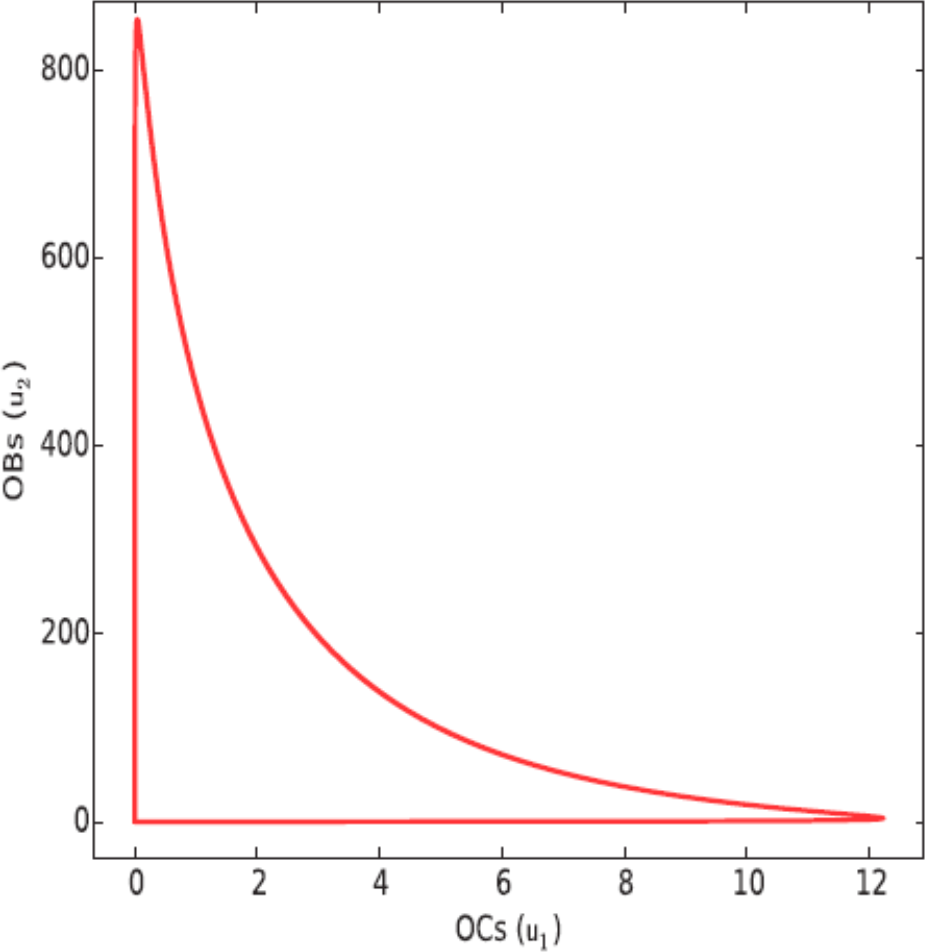
\includegraphics[width=.9\textwidth, keepaspectratio]{%
					./IMAGES/ComparacionDeModelos/pfSilvia.png}
		%\end{textblock*}	
	\end{columns}	
\end{frame}
%%%%%%%%%%%%%%%%%%%%%%%%%%%%%%%%%%%%%%%%%%%%%%%%%%%%%%%%%%%%%%%
\begin{frame}[plain]{Comparación de Fases}
	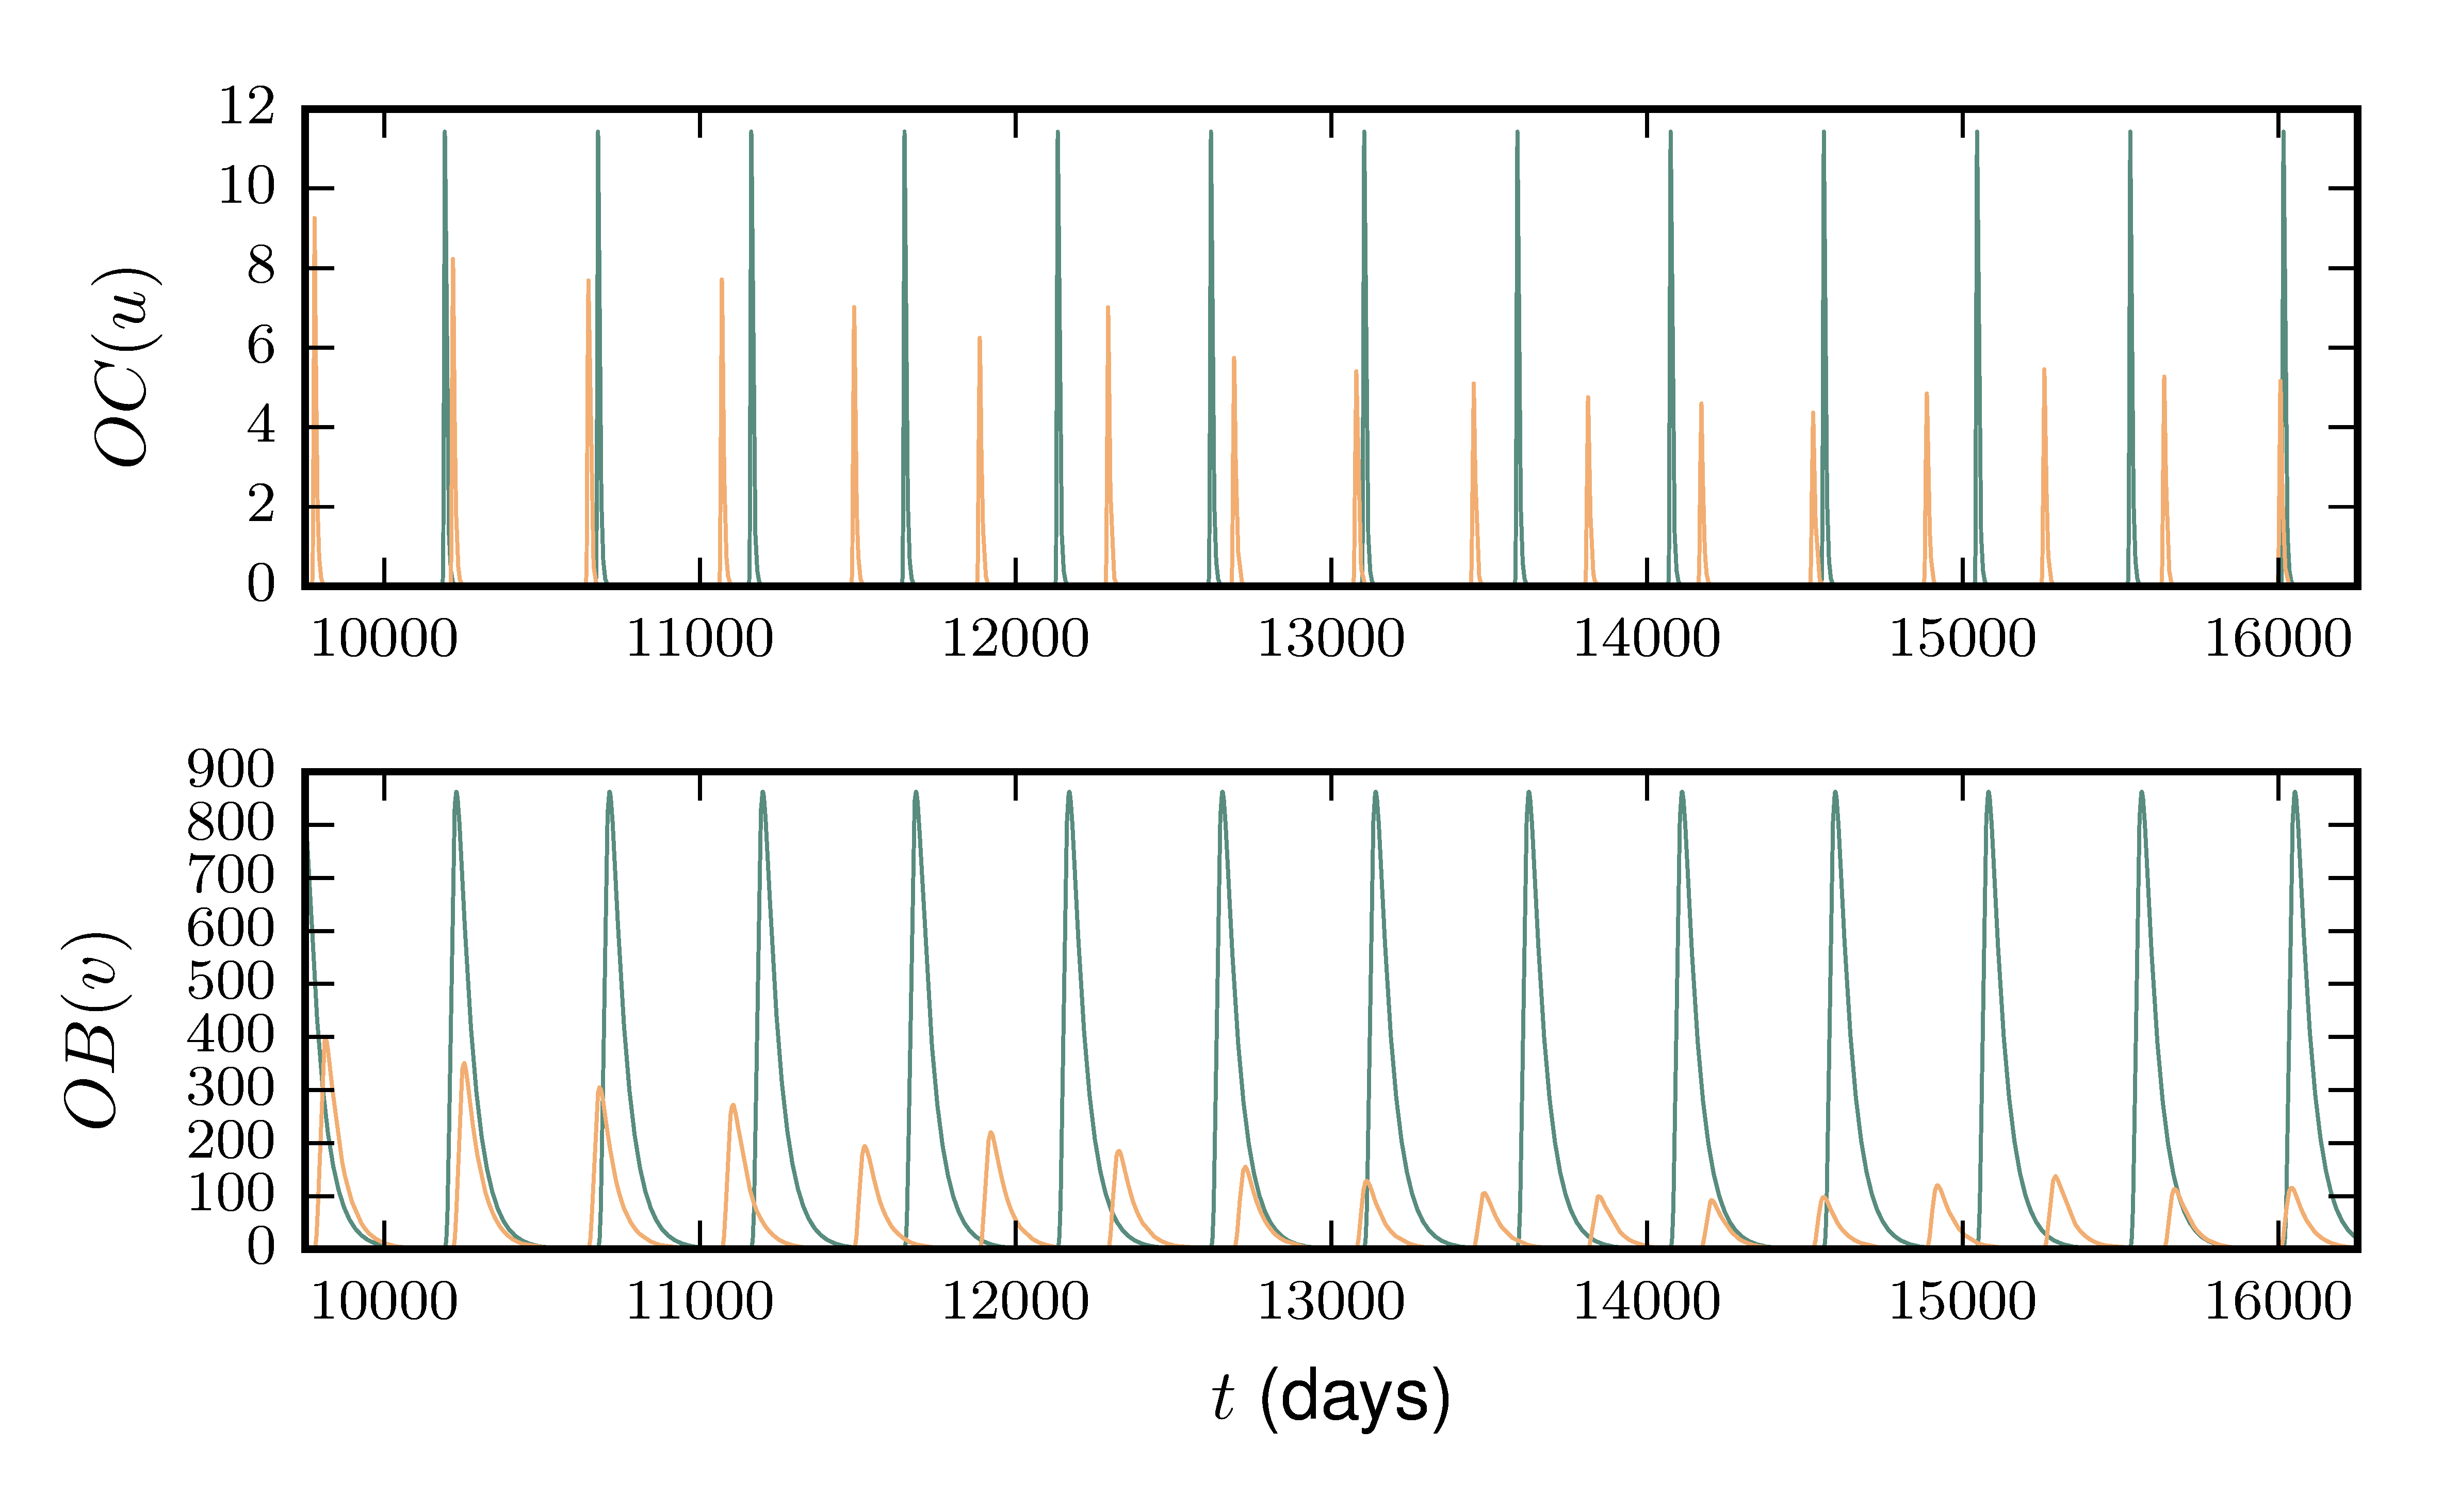
\includegraphics[width=\textwidth,keepaspectratio]{%
		./IMAGES/LongShortTime/ComparacionDeFase.png}
\end{frame}
%%%%%%%%%%%%%%%%%%%%%%%%%%%%%%%%%%%%%%%%%%%%%%%%%%%%%%%%%%%%%%%
\begin{frame}[plain]{PF tiempo corto (7 años) vs timpo largo (80-90 años)} 
	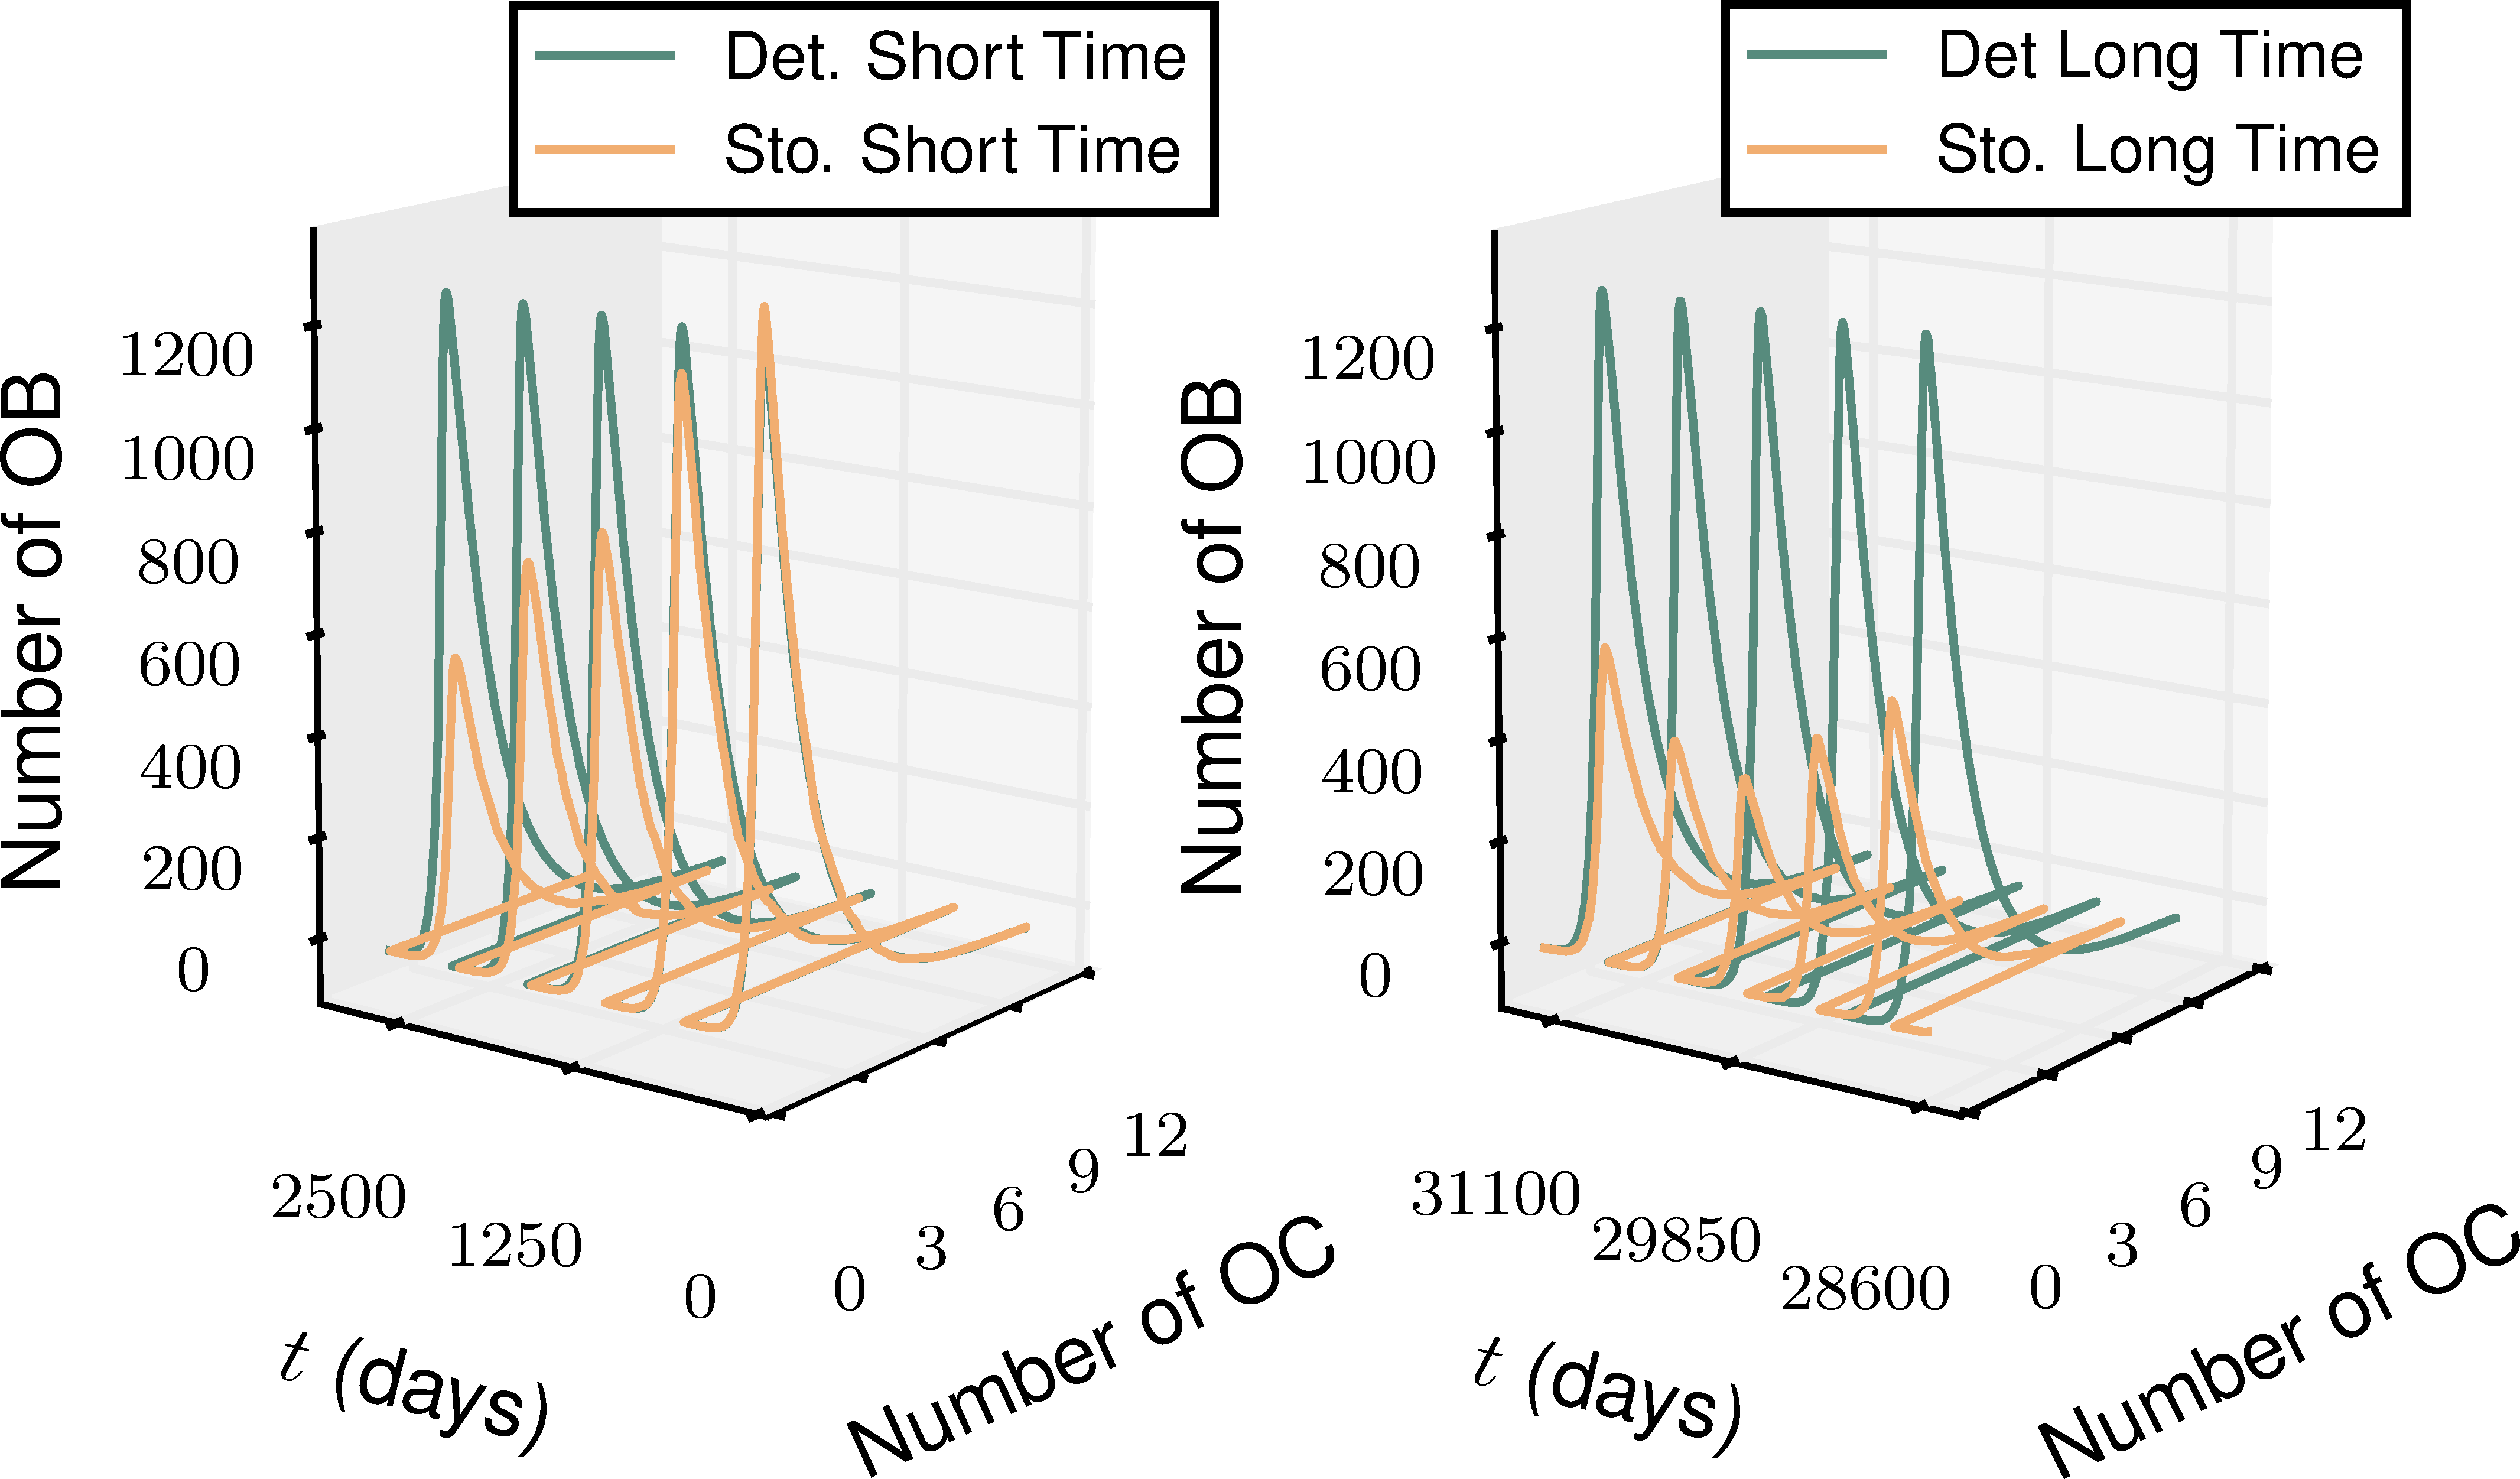
\includegraphics[width=\textwidth,keepaspectratio]{%
		%./IMAGES/LongShortTime/PhasePotrait3d(a).png
		./IMAGES/LongShortTime/ComparacionDePlanosFase.png%
		}
\end{frame}
%%%%%%%%%%%%%%%%%%%%%%%%%%%%%%%%%%%%%%%%%%%%%%%%%%%%%%%%%%%%%%%
\begin{frame}[plain]{Oscilaciones en torno a $\xi_i$}
	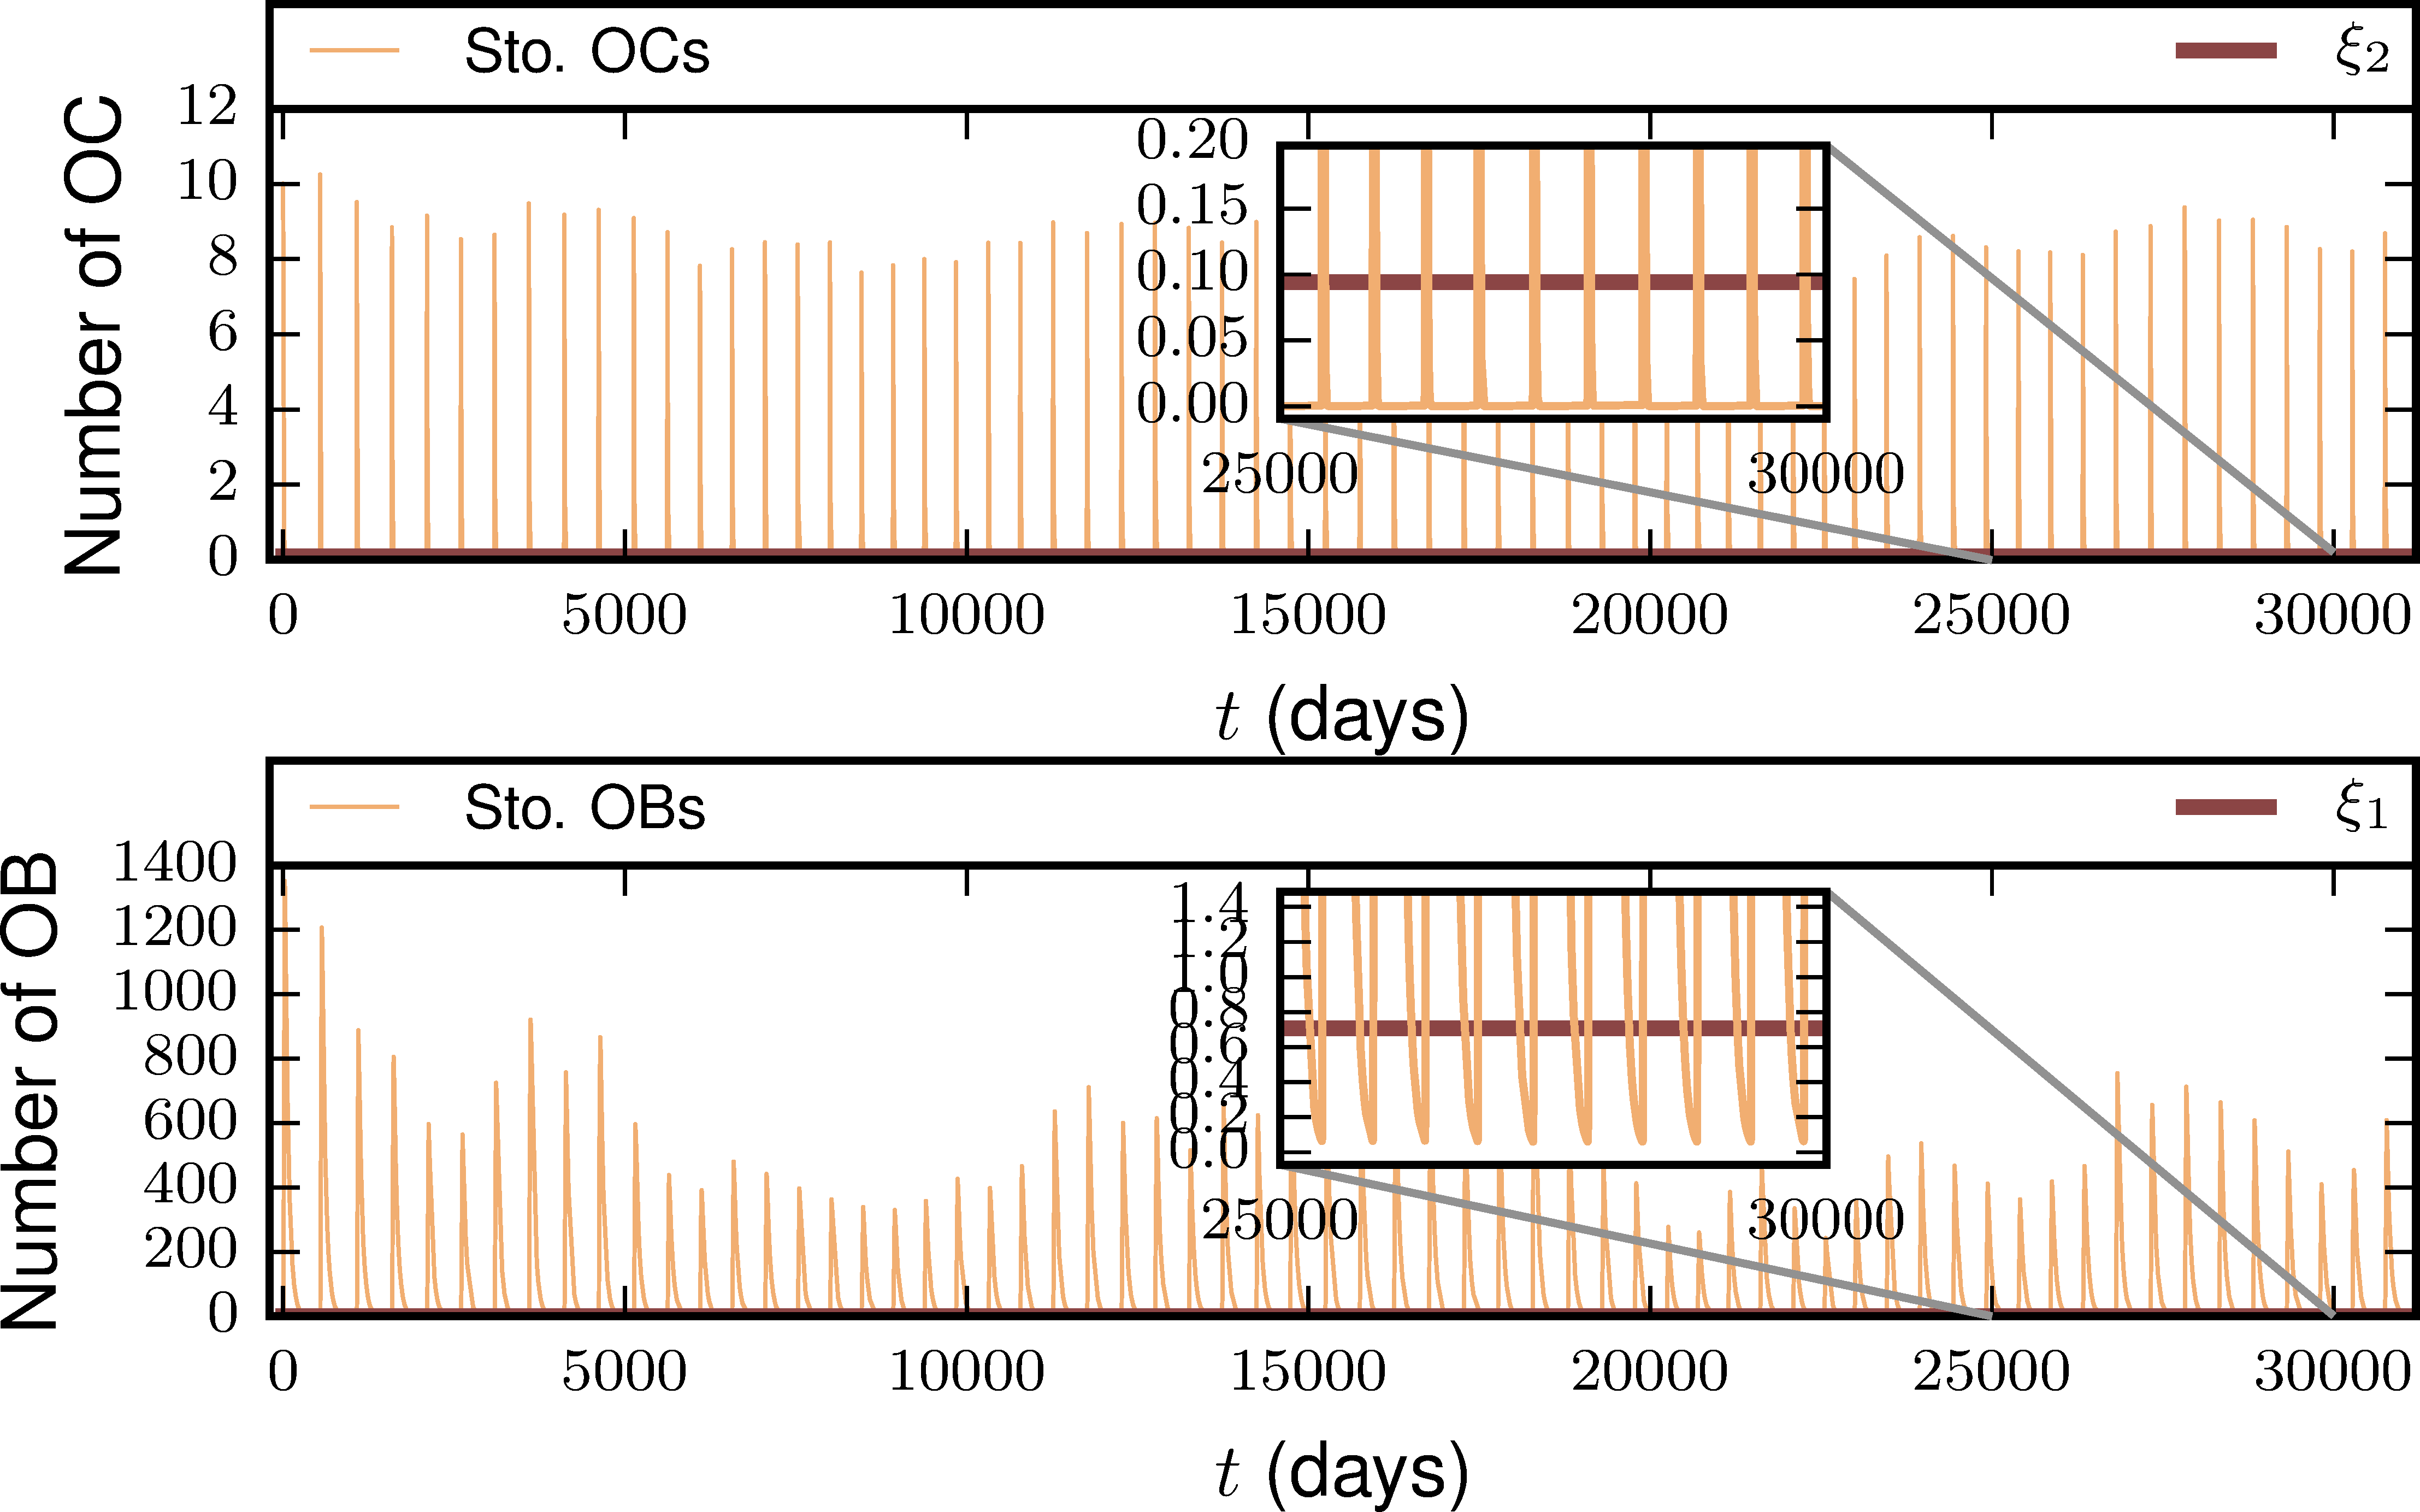
\includegraphics[width=\textwidth,keepaspectratio]{%
		%./IMAGES/LongShortTime/PhasePotrait3d(b).png
		./IMAGES/LongShortTime/OscilacionesXi1Xi2.png%
		}
\end{frame}
%%%%%%%%%%%%%%%%%%%%%%%%%%%%%%%%%%%%%%%%%%%%%%%%%%%%%%%%%%%%%%%
\begin{frame}[plain]{Trayectoria larga y  masa osea}
	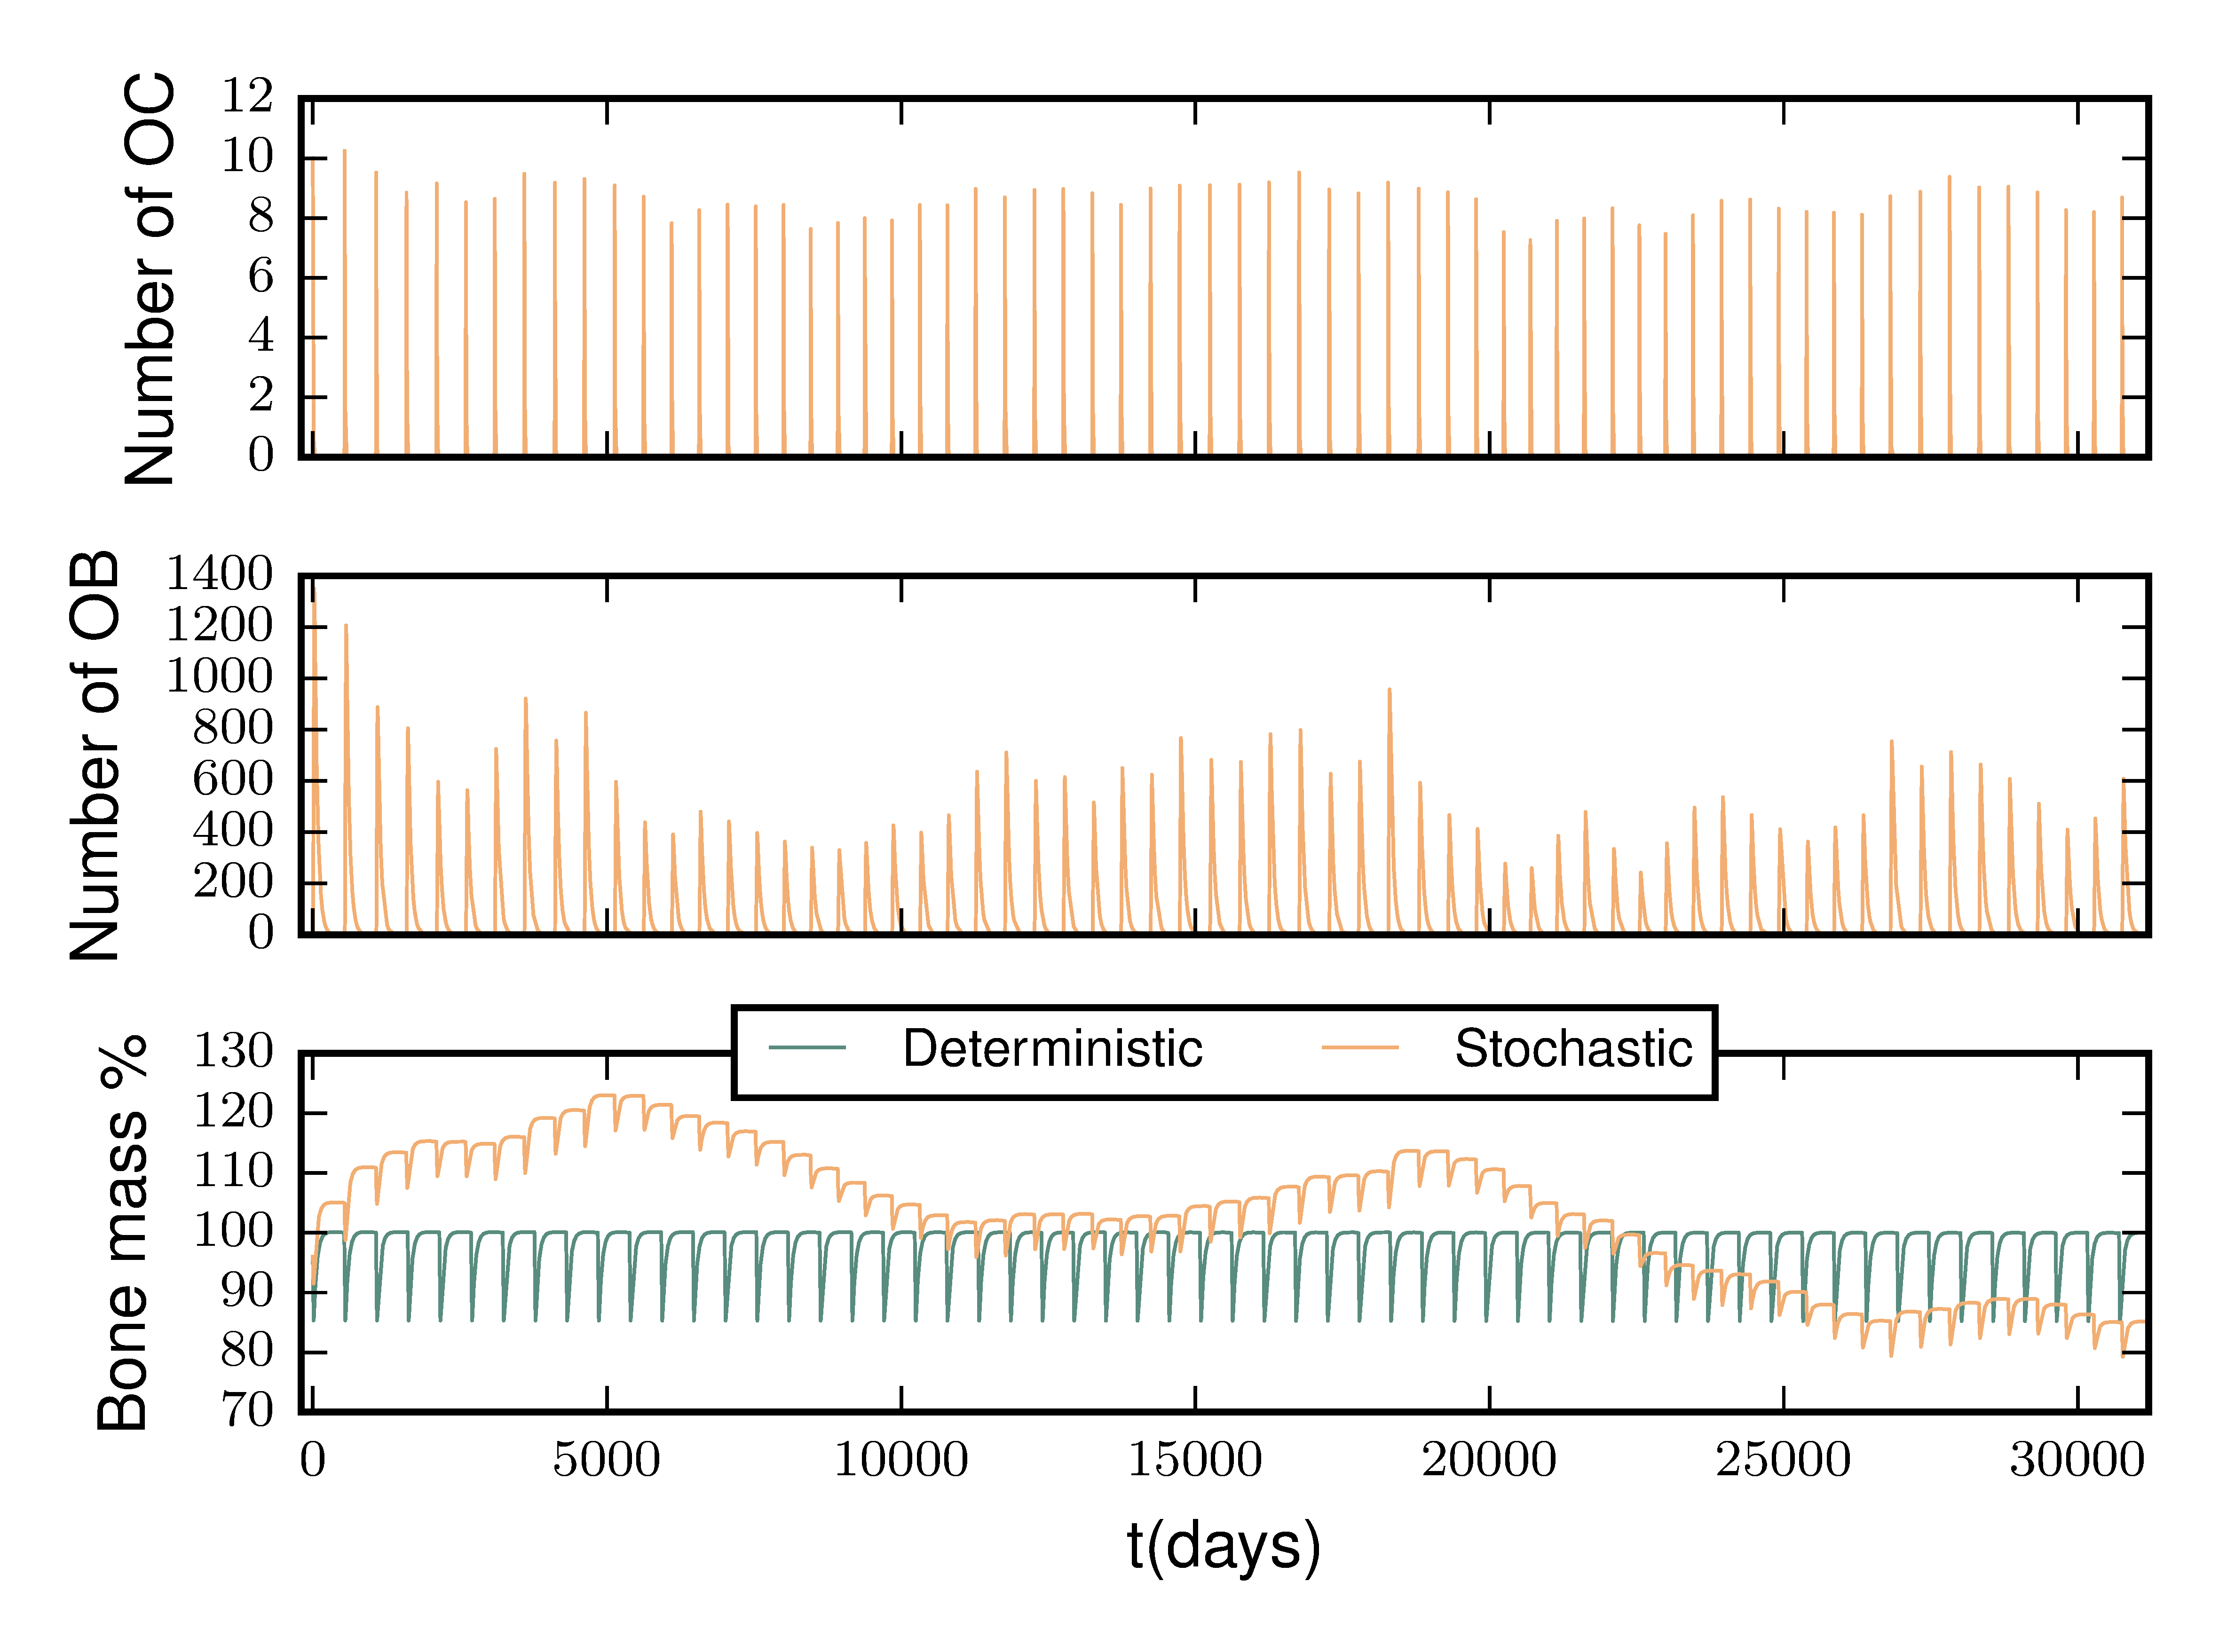
\includegraphics[width=\textwidth,keepaspectratio]{%
		./IMAGES/LongShortTime/longPahtBoneMass.png}
\end{frame}
%%%%%%%%%%%%%%%%%%%%%%%%%%%%%%%%%%%%%%%%%%%%%%%%%%%%%%%%%%%%%%%
\begin{frame}[plain]{Momentos a tiempo corto (13 años)}
	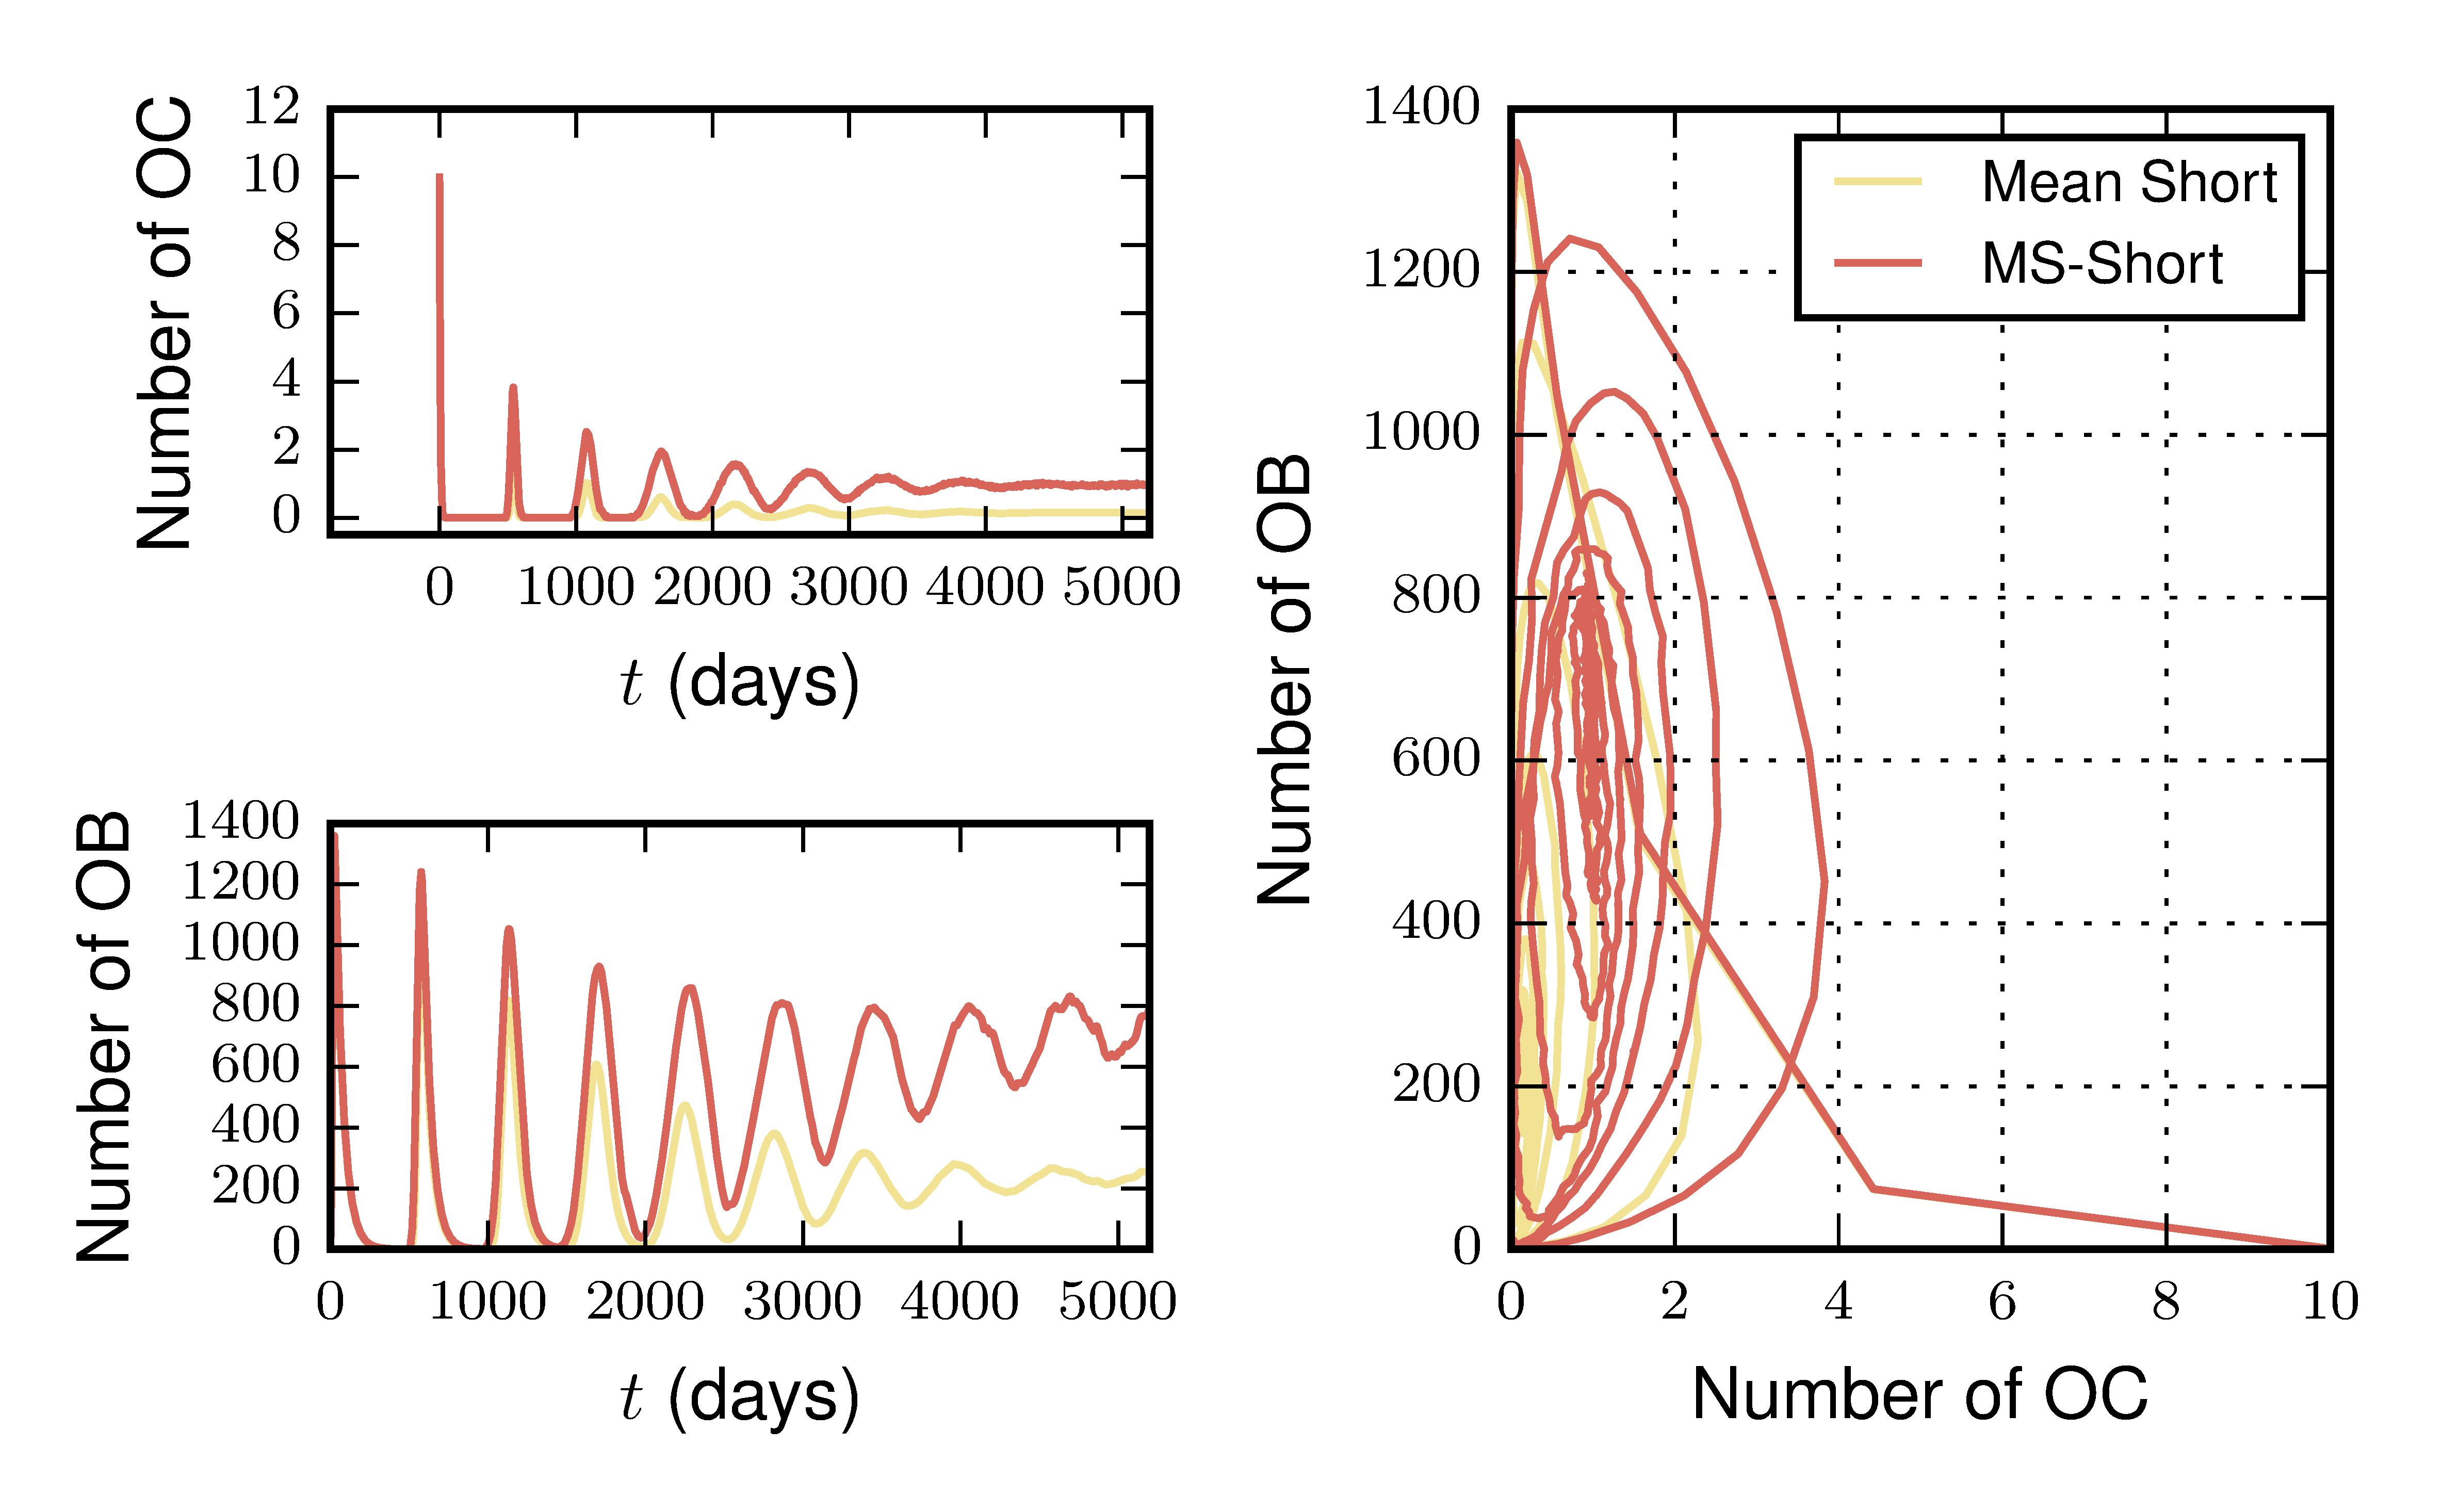
\includegraphics[width=\textwidth,keepaspectratio]{%
		./IMAGES/LongShortTime/shortTimeMoments.png}
\end{frame}
%%%%%%%%%%%%%%%%%%%%%%%%%%%%%%%%%%%%%%%%%%%%%%%%%%%%%%%%%%%%%%%
\begin{frame}[plain]{Momentos a tiempo largo}
	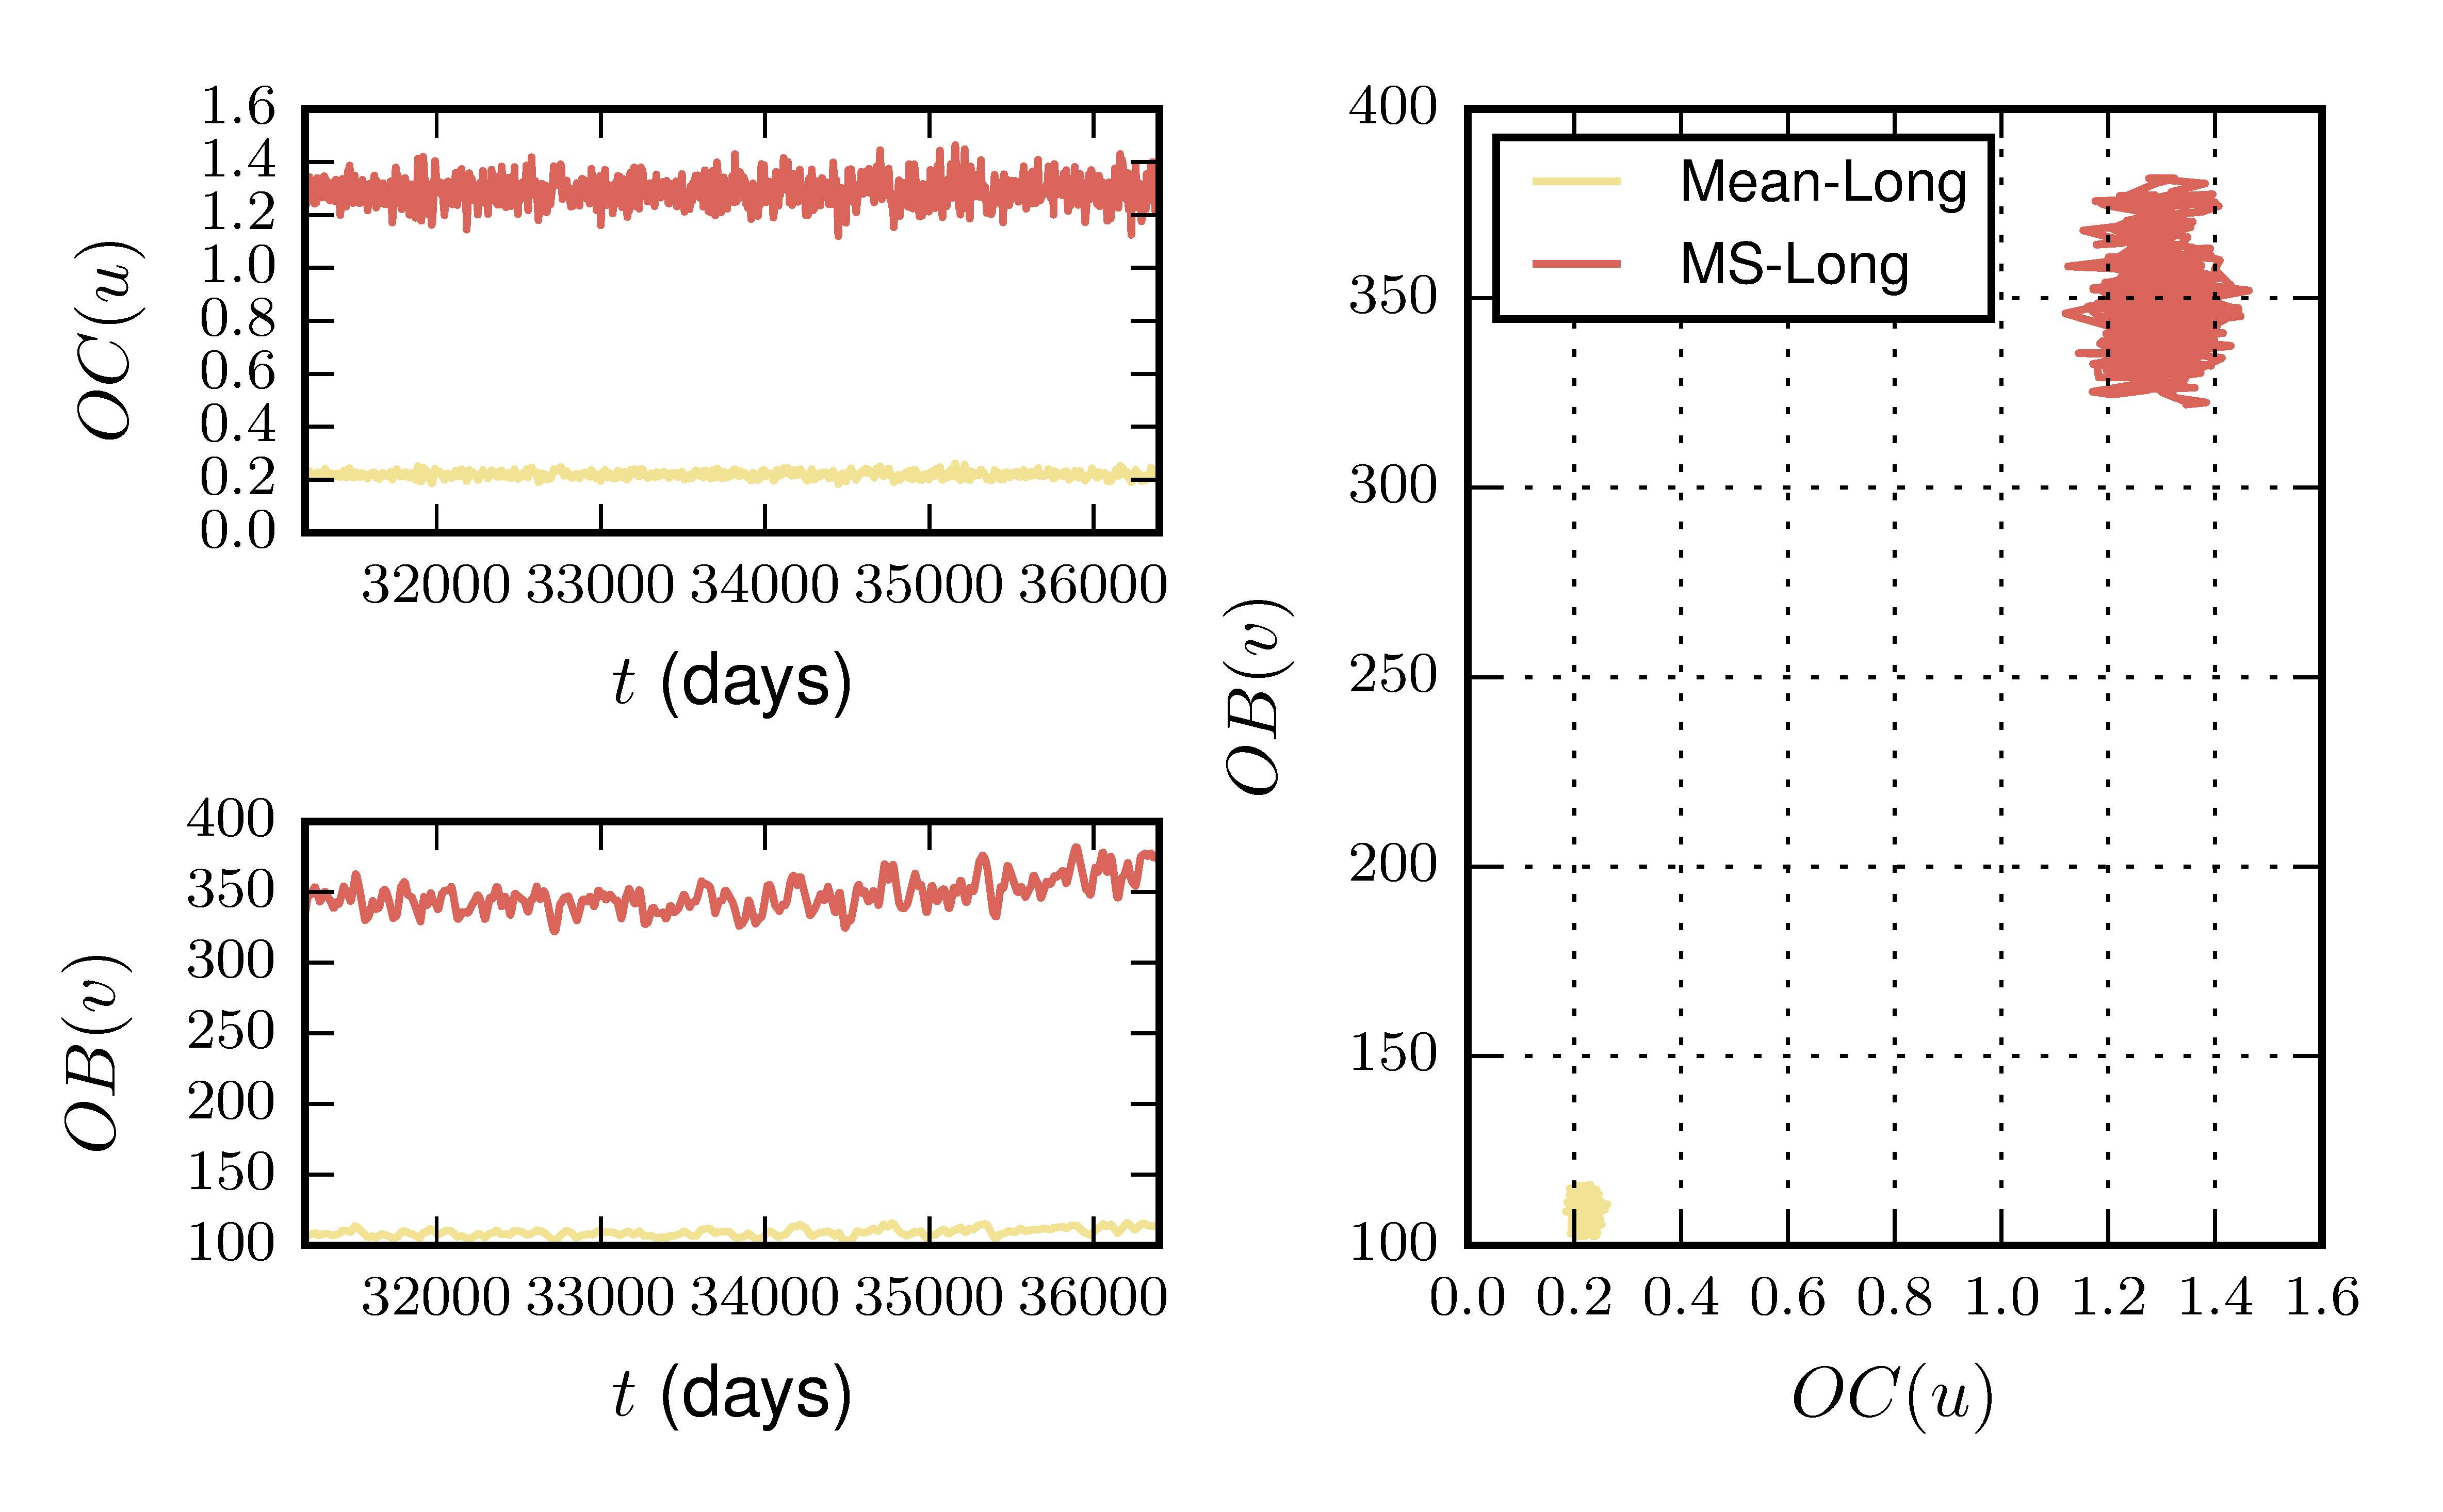
\includegraphics[width=\textwidth,keepaspectratio]{%
		./IMAGES/LongShortTime/longTimeMoments.png}
\end{frame}
%%%%%%%%%%%%%%%%%%%%%%%%%%%%%%%%%%%%%%%%%%%%%%%%%%%%%%%%%%%%%%%

    \section{Comentarios Finales}
        \begin{frame}[plain]
	\only<1-3>{
	\begin{textblock*}{100mm}(10mm, 40mm)
			\begin{block}{Sometido}    
					\begin{bibunit}[alpha]
					\nocite{Jerez2017}
				%\biblio{CharlaBib.bib}
				\putbib
			\end{bibunit}
			\end{block}   
	\end{textblock*}
	}
 	\only<2>{
		\begin{textblock*}{60mm}(40mm, 20mm)
			\Huge Gracias!!!
		\end{textblock*}
 	}
\end{frame}
    \appendix
        \begin{textblock*}{100mm}(10mm, 40mm)
    \begin{block}{Sometido}    
        \begin{bibunit}[alpha]
	       \nocite{Jerez2017}
		  %\biblio{CharlaBib.bib}
		  \putbib
	   \end{bibunit}
    \end{block}    
\end{textblock*} 
\end{document}
